\documentclass[]{book}
\usepackage{lmodern}
\usepackage{amssymb,amsmath}
\usepackage{ifxetex,ifluatex}
\usepackage{fixltx2e} % provides \textsubscript
\ifnum 0\ifxetex 1\fi\ifluatex 1\fi=0 % if pdftex
  \usepackage[T1]{fontenc}
  \usepackage[utf8]{inputenc}
\else % if luatex or xelatex
  \ifxetex
    \usepackage{mathspec}
  \else
    \usepackage{fontspec}
  \fi
  \defaultfontfeatures{Ligatures=TeX,Scale=MatchLowercase}
\fi
% use upquote if available, for straight quotes in verbatim environments
\IfFileExists{upquote.sty}{\usepackage{upquote}}{}
% use microtype if available
\IfFileExists{microtype.sty}{%
\usepackage{microtype}
\UseMicrotypeSet[protrusion]{basicmath} % disable protrusion for tt fonts
}{}
\usepackage[margin=1in]{geometry}
\usepackage{hyperref}
\hypersetup{unicode=true,
            pdftitle={DALEX: Descriptive mAchine Learning EXplanations},
            pdfauthor={Przemysław Biecek},
            pdfborder={0 0 0},
            breaklinks=true}
\urlstyle{same}  % don't use monospace font for urls
\usepackage{natbib}
\bibliographystyle{apalike}
\usepackage{color}
\usepackage{fancyvrb}
\newcommand{\VerbBar}{|}
\newcommand{\VERB}{\Verb[commandchars=\\\{\}]}
\DefineVerbatimEnvironment{Highlighting}{Verbatim}{commandchars=\\\{\}}
% Add ',fontsize=\small' for more characters per line
\usepackage{framed}
\definecolor{shadecolor}{RGB}{248,248,248}
\newenvironment{Shaded}{\begin{snugshade}}{\end{snugshade}}
\newcommand{\AlertTok}[1]{\textcolor[rgb]{0.94,0.16,0.16}{#1}}
\newcommand{\AnnotationTok}[1]{\textcolor[rgb]{0.56,0.35,0.01}{\textbf{\textit{#1}}}}
\newcommand{\AttributeTok}[1]{\textcolor[rgb]{0.77,0.63,0.00}{#1}}
\newcommand{\BaseNTok}[1]{\textcolor[rgb]{0.00,0.00,0.81}{#1}}
\newcommand{\BuiltInTok}[1]{#1}
\newcommand{\CharTok}[1]{\textcolor[rgb]{0.31,0.60,0.02}{#1}}
\newcommand{\CommentTok}[1]{\textcolor[rgb]{0.56,0.35,0.01}{\textit{#1}}}
\newcommand{\CommentVarTok}[1]{\textcolor[rgb]{0.56,0.35,0.01}{\textbf{\textit{#1}}}}
\newcommand{\ConstantTok}[1]{\textcolor[rgb]{0.00,0.00,0.00}{#1}}
\newcommand{\ControlFlowTok}[1]{\textcolor[rgb]{0.13,0.29,0.53}{\textbf{#1}}}
\newcommand{\DataTypeTok}[1]{\textcolor[rgb]{0.13,0.29,0.53}{#1}}
\newcommand{\DecValTok}[1]{\textcolor[rgb]{0.00,0.00,0.81}{#1}}
\newcommand{\DocumentationTok}[1]{\textcolor[rgb]{0.56,0.35,0.01}{\textbf{\textit{#1}}}}
\newcommand{\ErrorTok}[1]{\textcolor[rgb]{0.64,0.00,0.00}{\textbf{#1}}}
\newcommand{\ExtensionTok}[1]{#1}
\newcommand{\FloatTok}[1]{\textcolor[rgb]{0.00,0.00,0.81}{#1}}
\newcommand{\FunctionTok}[1]{\textcolor[rgb]{0.00,0.00,0.00}{#1}}
\newcommand{\ImportTok}[1]{#1}
\newcommand{\InformationTok}[1]{\textcolor[rgb]{0.56,0.35,0.01}{\textbf{\textit{#1}}}}
\newcommand{\KeywordTok}[1]{\textcolor[rgb]{0.13,0.29,0.53}{\textbf{#1}}}
\newcommand{\NormalTok}[1]{#1}
\newcommand{\OperatorTok}[1]{\textcolor[rgb]{0.81,0.36,0.00}{\textbf{#1}}}
\newcommand{\OtherTok}[1]{\textcolor[rgb]{0.56,0.35,0.01}{#1}}
\newcommand{\PreprocessorTok}[1]{\textcolor[rgb]{0.56,0.35,0.01}{\textit{#1}}}
\newcommand{\RegionMarkerTok}[1]{#1}
\newcommand{\SpecialCharTok}[1]{\textcolor[rgb]{0.00,0.00,0.00}{#1}}
\newcommand{\SpecialStringTok}[1]{\textcolor[rgb]{0.31,0.60,0.02}{#1}}
\newcommand{\StringTok}[1]{\textcolor[rgb]{0.31,0.60,0.02}{#1}}
\newcommand{\VariableTok}[1]{\textcolor[rgb]{0.00,0.00,0.00}{#1}}
\newcommand{\VerbatimStringTok}[1]{\textcolor[rgb]{0.31,0.60,0.02}{#1}}
\newcommand{\WarningTok}[1]{\textcolor[rgb]{0.56,0.35,0.01}{\textbf{\textit{#1}}}}
\usepackage{longtable,booktabs}
\usepackage{graphicx,grffile}
\makeatletter
\def\maxwidth{\ifdim\Gin@nat@width>\linewidth\linewidth\else\Gin@nat@width\fi}
\def\maxheight{\ifdim\Gin@nat@height>\textheight\textheight\else\Gin@nat@height\fi}
\makeatother
% Scale images if necessary, so that they will not overflow the page
% margins by default, and it is still possible to overwrite the defaults
% using explicit options in \includegraphics[width, height, ...]{}
\setkeys{Gin}{width=\maxwidth,height=\maxheight,keepaspectratio}
\IfFileExists{parskip.sty}{%
\usepackage{parskip}
}{% else
\setlength{\parindent}{0pt}
\setlength{\parskip}{6pt plus 2pt minus 1pt}
}
\setlength{\emergencystretch}{3em}  % prevent overfull lines
\providecommand{\tightlist}{%
  \setlength{\itemsep}{0pt}\setlength{\parskip}{0pt}}
\setcounter{secnumdepth}{5}
% Redefines (sub)paragraphs to behave more like sections
\ifx\paragraph\undefined\else
\let\oldparagraph\paragraph
\renewcommand{\paragraph}[1]{\oldparagraph{#1}\mbox{}}
\fi
\ifx\subparagraph\undefined\else
\let\oldsubparagraph\subparagraph
\renewcommand{\subparagraph}[1]{\oldsubparagraph{#1}\mbox{}}
\fi

%%% Use protect on footnotes to avoid problems with footnotes in titles
\let\rmarkdownfootnote\footnote%
\def\footnote{\protect\rmarkdownfootnote}

%%% Change title format to be more compact
\usepackage{titling}

% Create subtitle command for use in maketitle
\newcommand{\subtitle}[1]{
  \posttitle{
    \begin{center}\large#1\end{center}
    }
}

\setlength{\droptitle}{-2em}

  \title{DALEX: Descriptive mAchine Learning EXplanations}
    \pretitle{\vspace{\droptitle}\centering\huge}
  \posttitle{\par}
    \author{Przemysław Biecek}
    \preauthor{\centering\large\emph}
  \postauthor{\par}
      \predate{\centering\large\emph}
  \postdate{\par}
    \date{2018-06-19}

\usepackage{booktabs}
\usepackage{amsthm}
\makeatletter
\def\thm@space@setup{%
  \thm@preskip=8pt plus 2pt minus 4pt
  \thm@postskip=\thm@preskip
}
\makeatother

\usepackage{amsthm}
\newtheorem{theorem}{Theorem}[chapter]
\newtheorem{lemma}{Lemma}[chapter]
\theoremstyle{definition}
\newtheorem{definition}{Definition}[chapter]
\newtheorem{corollary}{Corollary}[chapter]
\newtheorem{proposition}{Proposition}[chapter]
\theoremstyle{definition}
\newtheorem{example}{Example}[chapter]
\theoremstyle{definition}
\newtheorem{exercise}{Exercise}[chapter]
\theoremstyle{remark}
\newtheorem*{remark}{Remark}
\newtheorem*{solution}{Solution}
\begin{document}
\maketitle

{
\setcounter{tocdepth}{1}
\tableofcontents
}
\hypertarget{introduction}{%
\chapter{Introduction}\label{introduction}}

\emph{Machine Learning} (ML) models have a wide range of applications in
classification or regression problems. Due to the increasing
computational power of computers and complexity of data sources, ML
models are becoming more and more sophisticated. Models created with the
use of techniques such as boosting or bagging of neural networks are
parametrized by thousands of coefficients. They are obscure; it is hard
to trace the link between input variables and model outcomes - in fact
they are treated as black boxes. They are used because of their
elasticity and high performance, but their deficiency in
interpretability is one of their weakest sides.

In many applications we need to know, understand or prove how the input
variables are used in the model. We need to know the impact of
particular variables on the final model predictions. Thus we need tools
that extract useful information from thousands of model parameters.

DALEX \citep[see][]{DALEX} is an R \citep{RcoreT} library with such
tools. DALEX helps to understand the way complex models work. In this
document we show two typical use-cases for DALEX: one case will increase
our understanding of a model, while the other will increase our
understanding of predictions for particular data points.

{Figure 1.1. Workflow of a typical machine learning modeling. A)
Modeling is a process in which domain knowledge and data are turned into
models. B) Models are used to generate predictions. C) Understanding of
a model structure may increase our knowledge, and in consequence it may
lead to a better model. DALEX helps here. D) Understanding of drivers
behind a particular model's predictions may help to correct wrong
decisions, and in consequence it leads to a better model. DALEX helps
here. }

\hypertarget{motivation}{%
\section{Motivation}\label{motivation}}

\emph{Machine Learning} is a vague name. There is some \emph{learning}
and some \emph{machines}, but what the heck is going on? What does it
really mean? Is it possible that the meaning of this term evolves over
time?

\begin{itemize}
\tightlist
\item
  A few years ago I would say that the term refers to \emph{machines
  learning from humans}. In the supervised learning problems, a human
  being creates a labeled dataset and machines are tuned/trained to
  predict correct labels from data.
\item
  Recently we have more and more examples of \emph{machines that are
  learning from other machines}. Self-playing neural nets like AlphaGo
  Zero \citep{AlphaGoZero} learn from themselves with blazing speed.
  Humans are involved in designing the learning environment but the
  labeling turns out to be very expensive or not feasible, and we are
  looking for other ways to learn from partial labels, fuzzy labels, or
  no labels at all.
\item
  I could imagine that in close future \emph{humans will learn from
  machines}. Well trained black-boxes may teach us how to be better at
  playing Go, how to be better at reading PET images (Positron-Emission
  Tomography images), or how to be better at diagnosing patients.
\end{itemize}

As the human supervision over learning is decreasing over time, the
understanding of black-boxes is more important. To make this future
possible, we need tools that extract useful information from black-box
models.

DALEX is \emph{the tool} for this.

\hypertarget{why-dalex}{%
\subsection{Why DALEX?}\label{why-dalex}}

In recent years we have been observing an increasing interest in tools
for knowledge extraction from complex machine learning models, see
\citep{Strumbelj}, \citep{nnet_vis}, \citep{magix},
\citep{Zeiler_Fergus_2014}.

There are some very useful R packages that may be used for knowledge
extraction from R models, see for example \texttt{pdp} \citep{pdp},
\texttt{ALEPlot} \citep{ALEPlot}, \texttt{randomForestExplainer}
\citep{randomForestExplainer}, \texttt{xgboostExplainer}
\citep{xgboostExplainer}, \texttt{live} \citep{live} and others.

Do we need yet another R package to better understand ML models? I think
so. There are some features available in the DALEX package which make it
unique.

\begin{itemize}
\tightlist
\item
  Scope. DALEX is a wrapper for a large number of very good tools /
  model explainers. It offers a wide range of state-of-the-art
  techniques for model exploration. Some of these techniques are more
  useful for understanding model predictions; other techniques are more
  handy for understanding model structure.
\item
  Consistency. DALEX offers a consistent grammar across various
  techniques for model explanation. It's a wrapper that smoothes
  differences across different R packages.
\item
  Model agnostic. DALEX explainers are model agnostic. One can use them
  for linear models, tree ensembles, or other structures, hence we are
  not limited to any particular family of black-box models.
\item
  Model comparisons. One can learn a lot from a single black-box model,
  but one can learn much more by contrasting models with different
  structures, like linear models with ensembles of trees. All DALEX
  explainers support model comparisons.
\item
  Visual consistency. Each DALEX explainer can be plotted with the
  generic \texttt{plot()} function. These visual explanations are based
  on \texttt{ggplot2} \citep{ggplot2} package, which generates elegant,
  customizable, and consistent graphs.
\end{itemize}

Chapter \ref{architecture} presents the overall architecture of the
DALEX package. Chapter \ref{modelUnderstanding} presents explainers that
explore global model performance and variable importance of feature
effects. Chapter \ref{predictionUnderstanding} presents explainers that
explore feature attribution for single predictions of validation of a
model prediction's reliability.

In this document we focus on three primary use-cases for DALEX
explainers.

\hypertarget{to-validate}{%
\subsection{To validate}\label{to-validate}}

Explainers presented in Section \ref{modelPerformance} help in
understanding model performance and comparing performance of different
models.

Explainers presented in Section \ref{outlierDetection} help to identify
outliers or observations with particularly large residuals.

Explainers presented in Section \ref{predictionBreakdown} help to
understand which key features influence model predictions.

\hypertarget{to-understand}{%
\subsection{To understand}\label{to-understand}}

Explainers presented in Section \ref{featureImportance} help to
understand which variables are the most important in the model.
Explainers presented in Section \ref{predictionBreakdown} help to
understand which features influence single predictions. They are useful
in identifying key influencers behind the black-box.

Explainers presented in Section \ref{variableResponse} help to
understand how particular features affect model prediction.

\hypertarget{to-improve}{%
\subsection{To improve}\label{to-improve}}

Explainers presented in Section \ref{variableResponse} help to perform
feature engineering based on model conditional responses.

Explainers presented in Section \ref{predictionBreakdown} help to
understand which variables result in incorrect model decisions. These
explainers are useful in identifying and correcting biases in the
training data.

\hypertarget{trivia}{%
\section{Trivia}\label{trivia}}

{ 
\includegraphics{images/dalex01small.jpg} }

\href{https://en.wikipedia.org/wiki/Dalek}{The Daleks} are a fictional
extraterrestrial race portrayed in the
\href{https://en.wikipedia.org/wiki/Doctor_Who}{Doctor Who} BBC series.
Rather dim aliens, known to repeat the phrase \emph{Explain!} very
often. Daleks were engineered. They consist of live bodies closed in
tank-like robotic shells. They seem like nice mascots for explanations
concerning Machine Learning models.

\hypertarget{architecture}{%
\chapter{Architecture of DALEX}\label{architecture}}

DALEX's architecture is simple and consistent. Actually, there are only
three rules that should be remembered while using this tool.

\begin{itemize}
\tightlist
\item
  First - use the \texttt{explain()} function to enrich a black-box
  model with additional metadata required by explainers. Various
  explainers require various metadata. You may find their list in
  Section \ref{explainFunction}.
\item
  Second - use the explainer function that calculates required
  descriptions. Consecutive explainers are introduced in Chapters
  \ref{modelUnderstanding} and \ref{predictionUnderstanding}.
\item
  Third - use generic \texttt{print()} or \texttt{plot()} function to
  see the explainer. Both functions work for one or more models.
\end{itemize}

These three steps are presented in Figure 2.1.

{Figure 2.1. The overview of DALEX's architecture. \emph{A)} Any
predictive model with defined input \(x\) and output
\(y_{raw} \in \mathcal R\) may be used. \emph{B)} Models are first
enriched with additional metadata, such as a function that calculates
predictions, validation data, model label or other components. The
\texttt{explain()} function creates an object belonging to the
\texttt{explainer} class that is used in further processing. \emph{C)}
Specialized explainers calculate numerical summaries that can be plotted
with generic \texttt{plot()} function. }

\hypertarget{explainFunction}{%
\section{\texorpdfstring{The \texttt{explain()}
function}{The explain() function}}\label{explainFunction}}

DALEX is designed to work with various black-box models like tree
ensembles, linear models, neural networks etc. Unfortunately R packages
that create such models are very inconsistent. Different tools use
different interfaces to train, validate and use models. Two most popular
frameworks for machine learning are \texttt{mlr} \citep{mlr} and
\texttt{caret} \citep{caret}. Apart from them, dozens of R packages may
be used for modeling.

This is why as the first step DALEX wraps-up the black-box model with
meta-data that unifies model interfacing.

Below is a list of arguments required by the \texttt{explain()}
function.

\begin{verbatim}
explain(model, data, y, predict_function, 
               link, ..., label)
\end{verbatim}

\begin{itemize}
\tightlist
\item
  \texttt{model} - an R object, a model to be explained. \emph{Required
  by}: all explainers.
\item
  \texttt{data} - \texttt{data.frame} or \texttt{matrix}, a set that
  will be used for model validation. It should have the same structure
  as the dataset used for training. \emph{Required by}: model
  performance, variable importance. \emph{Default}: if possible, it
  should be extracted from the \texttt{model} object.
\item
  \texttt{y} - a numeric vector with true labels paired with
  observations in \texttt{data}. \emph{Required by}: variable
  importance. \emph{Default}: no default.
\item
  \texttt{predict\_function} - a function that takes two arguments:
  model and data, and returns numeric vector with predictions.
  Predictions should be calculated in the same scale as the \texttt{y}
  labels. \emph{Required by}: all explainers. \emph{Default}: the
  generic \texttt{predict()} function.
\item
  \texttt{link\_function} - a transformation/link function that is
  applied to model predictions. \emph{Required by}: variable effect.
  \emph{Default}: the identity \texttt{I()} function.
\item
  \texttt{label} - a character, a name of the model that will be used in
  plots. \emph{Required by}: plots. \emph{Default}: extracted from the
  \texttt{class} attribute of the \texttt{model}.
\end{itemize}

{Figure 2.2. The \texttt{explain()} function embeds \texttt{model},
validation \texttt{data} and \texttt{y} labels in a container. Model is
accessed via universal interface specified by
\texttt{predict\_function()} and \texttt{link\_function()}. The
\texttt{label} field contains a unique name of the model. }

The next section introduces use cases of regression. It will help to
understand how to use the \texttt{explain()} function and for what
purposes. Same functions may be used for binary classification.

\hypertarget{useCaseApartmetns}{%
\section{Use case: Regression. Apartment prices in
Warsaw}\label{useCaseApartmetns}}

To illustrate applications of DALEX to regression problems we will use
an artificial dataset \texttt{apartments} available in the
\texttt{DALEX} package. Our goal is to predict the price per square
meter of an apartment based on selected features such as construction
year, surface, floor, number of rooms, district. It should be noted that
four of these variables are continuous while the fifth one is a
categorical one. Prices are given in Euro.

\begin{Shaded}
\begin{Highlighting}[]
\KeywordTok{library}\NormalTok{(}\StringTok{"DALEX"}\NormalTok{)}
\KeywordTok{head}\NormalTok{(apartments)}
\end{Highlighting}
\end{Shaded}

\textbackslash{}begin\{table\}

\textbackslash{}caption\{(\#tab:hr\_data)Artificial dataset about
apartment prices in Warsaw. The goal here is to predict the price per
square meter for a new apartment.\} \centering

\begin{tabular}[t]{r|r|r|r|r|l}
\hline
m2.price & construction.year & surface & floor & no.rooms & district\\
\hline
5897 & 1953 & 25 & 3 & 1 & Srodmiescie\\
\hline
1818 & 1992 & 143 & 9 & 5 & Bielany\\
\hline
3643 & 1937 & 56 & 1 & 2 & Praga\\
\hline
3517 & 1995 & 93 & 7 & 3 & Ochota\\
\hline
3013 & 1992 & 144 & 6 & 5 & Mokotow\\
\hline
5795 & 1926 & 61 & 6 & 2 & Srodmiescie\\
\hline
\end{tabular}

\textbackslash{}end\{table\}

\hypertarget{model-1-linear-regression}{%
\subsection{Model 1: Linear
regression}\label{model-1-linear-regression}}

The first model is based on linear regression. It will be a simple model
without any feature engineering.

\begin{Shaded}
\begin{Highlighting}[]
\NormalTok{apartments_lm_model <-}\StringTok{ }\KeywordTok{lm}\NormalTok{(m2.price }\OperatorTok{~}\StringTok{ }\NormalTok{construction.year }\OperatorTok{+}\StringTok{ }\NormalTok{surface }\OperatorTok{+}\StringTok{ }\NormalTok{floor }\OperatorTok{+}\StringTok{ }
\StringTok{                         }\NormalTok{no.rooms }\OperatorTok{+}\StringTok{ }\NormalTok{district, }\DataTypeTok{data =}\NormalTok{ apartments)}
\KeywordTok{summary}\NormalTok{(apartments_lm_model)}
\end{Highlighting}
\end{Shaded}

\begin{verbatim}
## 
## Call:
## lm(formula = m2.price ~ construction.year + surface + floor + 
##     no.rooms + district, data = apartments)
## 
## Residuals:
##    Min     1Q Median     3Q    Max 
## -247.5 -202.8 -172.8  381.4  469.0 
## 
## Coefficients:
##                      Estimate Std. Error t value Pr(>|t|)    
## (Intercept)         5020.1391   682.8721   7.352 4.11e-13 ***
## construction.year     -0.2290     0.3483  -0.657   0.5110    
## surface              -10.2378     0.5778 -17.720  < 2e-16 ***
## floor                -99.4820     3.0874 -32.222  < 2e-16 ***
## no.rooms             -37.7299    15.8440  -2.381   0.0174 *  
## districtBielany       17.2144    40.4502   0.426   0.6705    
## districtMokotow      918.3802    39.4386  23.286  < 2e-16 ***
## districtOchota       926.2540    40.5279  22.855  < 2e-16 ***
## districtPraga        -37.1047    40.8930  -0.907   0.3644    
## districtSrodmiescie 2080.6110    40.0149  51.996  < 2e-16 ***
## districtUrsus         29.9419    39.7249   0.754   0.4512    
## districtUrsynow      -18.8651    39.7565  -0.475   0.6352    
## districtWola         -16.8912    39.6283  -0.426   0.6700    
## districtZoliborz     889.9735    40.4099  22.024  < 2e-16 ***
## ---
## Signif. codes:  0 '***' 0.001 '**' 0.01 '*' 0.05 '.' 0.1 ' ' 1
## 
## Residual standard error: 281.3 on 986 degrees of freedom
## Multiple R-squared:  0.905,  Adjusted R-squared:  0.9037 
## F-statistic: 722.5 on 13 and 986 DF,  p-value: < 2.2e-16
\end{verbatim}

We have also another \texttt{apartmentsTest} dataset that can be used
for validation of the model. Below is presented the mean square error
calculated on the basis of validation data.

\begin{Shaded}
\begin{Highlighting}[]
\NormalTok{predicted_mi2_lm <-}\StringTok{ }\KeywordTok{predict}\NormalTok{(apartments_lm_model, apartmentsTest)}
\KeywordTok{sqrt}\NormalTok{(}\KeywordTok{mean}\NormalTok{((predicted_mi2_lm }\OperatorTok{-}\StringTok{ }\NormalTok{apartmentsTest}\OperatorTok{$}\NormalTok{m2.price)}\OperatorTok{^}\DecValTok{2}\NormalTok{))}
\end{Highlighting}
\end{Shaded}

\begin{verbatim}
## [1] 283.0865
\end{verbatim}

To create an explainer for the regression model it is enough to use
\texttt{explain()} function with the \texttt{model}, \texttt{data} and
\texttt{y} parameters. In the next chapter we will show how to use this
explainer.

\begin{Shaded}
\begin{Highlighting}[]
\NormalTok{explainer_lm <-}\StringTok{ }\KeywordTok{explain}\NormalTok{(apartments_lm_model, }
                          \DataTypeTok{data =}\NormalTok{ apartmentsTest[,}\DecValTok{2}\OperatorTok{:}\DecValTok{6}\NormalTok{], }\DataTypeTok{y =}\NormalTok{ apartmentsTest}\OperatorTok{$}\NormalTok{m2.price)}
\end{Highlighting}
\end{Shaded}

\hypertarget{model-2-random-forest}{%
\subsection{Model 2: Random forest}\label{model-2-random-forest}}

The second model is based on the random forest. It's a very elastic
out-of-the-box model.

\begin{Shaded}
\begin{Highlighting}[]
\KeywordTok{library}\NormalTok{(}\StringTok{"randomForest"}\NormalTok{)}
\KeywordTok{set.seed}\NormalTok{(}\DecValTok{59}\NormalTok{)}

\NormalTok{apartments_rf_model <-}\StringTok{ }\KeywordTok{randomForest}\NormalTok{(m2.price }\OperatorTok{~}\StringTok{ }\NormalTok{construction.year }\OperatorTok{+}\StringTok{ }\NormalTok{surface }\OperatorTok{+}\StringTok{ }\NormalTok{floor }\OperatorTok{+}\StringTok{ }
\StringTok{                      }\NormalTok{no.rooms }\OperatorTok{+}\StringTok{ }\NormalTok{district, }\DataTypeTok{data =}\NormalTok{ apartments)}
\NormalTok{apartments_rf_model}
\end{Highlighting}
\end{Shaded}

\begin{verbatim}
## 
## Call:
##  randomForest(formula = m2.price ~ construction.year + surface +      floor + no.rooms + district, data = apartments) 
##                Type of random forest: regression
##                      Number of trees: 500
## No. of variables tried at each split: 1
## 
##           Mean of squared residuals: 82614.7
##                     % Var explained: 89.94
\end{verbatim}

Below you may see the mean square error calculated for
\texttt{apartmentsTest} dataset.

\begin{Shaded}
\begin{Highlighting}[]
\NormalTok{predicted_mi2_rf <-}\StringTok{ }\KeywordTok{predict}\NormalTok{(apartments_rf_model, apartmentsTest)}
\KeywordTok{sqrt}\NormalTok{(}\KeywordTok{mean}\NormalTok{((predicted_mi2_rf }\OperatorTok{-}\StringTok{ }\NormalTok{apartmentsTest}\OperatorTok{$}\NormalTok{m2.price)}\OperatorTok{^}\DecValTok{2}\NormalTok{))}
\end{Highlighting}
\end{Shaded}

\begin{verbatim}
## [1] 286.5357
\end{verbatim}

We will create an explainer also for the random forest model. In the
next chapter we will show how to use this explainer.

\begin{Shaded}
\begin{Highlighting}[]
\NormalTok{explainer_rf <-}\StringTok{ }\KeywordTok{explain}\NormalTok{(apartments_rf_model, }
                       \DataTypeTok{data =}\NormalTok{ apartmentsTest[,}\DecValTok{2}\OperatorTok{:}\DecValTok{6}\NormalTok{], }\DataTypeTok{y =}\NormalTok{ apartmentsTest}\OperatorTok{$}\NormalTok{m2.price)}
\end{Highlighting}
\end{Shaded}

\textbf{These two models have identical performance!} Which one should
be used?

\hypertarget{modelUnderstanding}{%
\chapter{Model understanding}\label{modelUnderstanding}}

In this chapter we introduce three groups of explainers that can be used
to boost our understanding of black-box models.

\begin{itemize}
\tightlist
\item
  Section \ref{modelPerformance} presents explainers for model
  performance. A single number may be misleading when we need to compare
  complex models. In this section you will also find plots that give
  more information about model performance in a consistent form.
\item
  Section \ref{featureImportance} presents explainers for variable
  importance. Knowing which variables are important allows us to
  validate the model and increase our understanding of the domain.
\item
  Section \ref{variableResponse} presents explainers for variable
  effect. You may find in it plots that summarize the relation between
  model response and particular variables.
\end{itemize}

All explainers are illustrated on the basis of two models fitted to the
\texttt{apartments} data.

\begin{Shaded}
\begin{Highlighting}[]
\KeywordTok{library}\NormalTok{(}\StringTok{"DALEX"}\NormalTok{)}
\NormalTok{apartments_lm_model <-}\StringTok{ }\KeywordTok{lm}\NormalTok{(m2.price }\OperatorTok{~}\StringTok{ }\NormalTok{construction.year }\OperatorTok{+}\StringTok{ }\NormalTok{surface }\OperatorTok{+}\StringTok{ }\NormalTok{floor }\OperatorTok{+}\StringTok{ }
\StringTok{                      }\NormalTok{no.rooms }\OperatorTok{+}\StringTok{ }\NormalTok{district, }\DataTypeTok{data =}\NormalTok{ apartments)}
\KeywordTok{library}\NormalTok{(}\StringTok{"randomForest"}\NormalTok{)}
\KeywordTok{set.seed}\NormalTok{(}\DecValTok{59}\NormalTok{)}
\NormalTok{apartments_rf_model <-}\StringTok{ }\KeywordTok{randomForest}\NormalTok{(m2.price }\OperatorTok{~}\StringTok{ }\NormalTok{construction.year }\OperatorTok{+}\StringTok{ }\NormalTok{surface }\OperatorTok{+}\StringTok{ }\NormalTok{floor }\OperatorTok{+}\StringTok{ }
\StringTok{                      }\NormalTok{no.rooms }\OperatorTok{+}\StringTok{ }\NormalTok{district, }\DataTypeTok{data =}\NormalTok{ apartments)}
\end{Highlighting}
\end{Shaded}

First we need to prepare wrappers for these models. They are in
\texttt{explainer\_lm} and \texttt{explainer\_rf} objects.

\begin{Shaded}
\begin{Highlighting}[]
\NormalTok{explainer_lm <-}\StringTok{ }\KeywordTok{explain}\NormalTok{(apartments_lm_model, }
                       \DataTypeTok{data =}\NormalTok{ apartmentsTest[,}\DecValTok{2}\OperatorTok{:}\DecValTok{6}\NormalTok{], }\DataTypeTok{y =}\NormalTok{ apartmentsTest}\OperatorTok{$}\NormalTok{m2.price)}
\NormalTok{explainer_rf <-}\StringTok{ }\KeywordTok{explain}\NormalTok{(apartments_rf_model, }
                       \DataTypeTok{data =}\NormalTok{ apartmentsTest[,}\DecValTok{2}\OperatorTok{:}\DecValTok{6}\NormalTok{], }\DataTypeTok{y =}\NormalTok{ apartmentsTest}\OperatorTok{$}\NormalTok{m2.price)}
\end{Highlighting}
\end{Shaded}

\hypertarget{modelPerformance}{%
\section{Model performance}\label{modelPerformance}}

As you may remember from the previous chapter, the
\href{https://en.wikipedia.org/wiki/Root_mean_square}{root mean square}
of residuals is identical for both considered models. Does it mean that
these models are equally good?

\begin{Shaded}
\begin{Highlighting}[]
\NormalTok{predicted_mi2_lm <-}\StringTok{ }\KeywordTok{predict}\NormalTok{(apartments_lm_model, apartmentsTest)}
\KeywordTok{sqrt}\NormalTok{(}\KeywordTok{mean}\NormalTok{((predicted_mi2_lm }\OperatorTok{-}\StringTok{ }\NormalTok{apartmentsTest}\OperatorTok{$}\NormalTok{m2.price)}\OperatorTok{^}\DecValTok{2}\NormalTok{))}
\end{Highlighting}
\end{Shaded}

\begin{verbatim}
## [1] 283.0865
\end{verbatim}

\begin{Shaded}
\begin{Highlighting}[]
\NormalTok{predicted_mi2_rf <-}\StringTok{ }\KeywordTok{predict}\NormalTok{(apartments_rf_model, apartmentsTest)}
\KeywordTok{sqrt}\NormalTok{(}\KeywordTok{mean}\NormalTok{((predicted_mi2_rf }\OperatorTok{-}\StringTok{ }\NormalTok{apartmentsTest}\OperatorTok{$}\NormalTok{m2.price)}\OperatorTok{^}\DecValTok{2}\NormalTok{))}
\end{Highlighting}
\end{Shaded}

\begin{verbatim}
## [1] 286.5357
\end{verbatim}

Function \texttt{model\_performance()} calculates predictions and
residuals for validation dataset \texttt{apartmentsTest}.

Generic function \texttt{print()} returns quantiles for residuals.

\begin{Shaded}
\begin{Highlighting}[]
\NormalTok{mp_lm <-}\StringTok{ }\KeywordTok{model_performance}\NormalTok{(explainer_lm)}
\NormalTok{mp_rf <-}\StringTok{ }\KeywordTok{model_performance}\NormalTok{(explainer_rf)}
\NormalTok{mp_lm}
\end{Highlighting}
\end{Shaded}

\begin{verbatim}
##        0%       10%       20%       30%       40%       50%       60% 
## -472.3560 -423.9131 -398.2811 -370.8841  161.2473  174.0677  184.1412 
##       70%       80%       90%      100% 
##  195.8834  209.2460  221.4659  257.2555
\end{verbatim}

\begin{Shaded}
\begin{Highlighting}[]
\NormalTok{mp_rf}
\end{Highlighting}
\end{Shaded}

\begin{verbatim}
##           0%          10%          20%          30%          40% 
## -1262.554308  -408.920183  -197.591180   -89.661883    -7.454146 
##          50%          60%          70%          80%          90% 
##    55.441061   108.398858   157.924244   218.241574   294.264602 
##         100% 
##   727.445065
\end{verbatim}

The generic \texttt{plot()} function shows reversed empirical cumulative
distribution function for absolute values from residuals. This function
presents a fraction of residuals larger than \texttt{x}. The figure
below shows that majority of residuals for the random forest is smaller
than residuals for the linear model, yet the small fraction of very
large residuals affects the root mean square.

\begin{Shaded}
\begin{Highlighting}[]
\KeywordTok{plot}\NormalTok{(mp_lm, mp_rf)}
\end{Highlighting}
\end{Shaded}

\begin{figure}
\centering
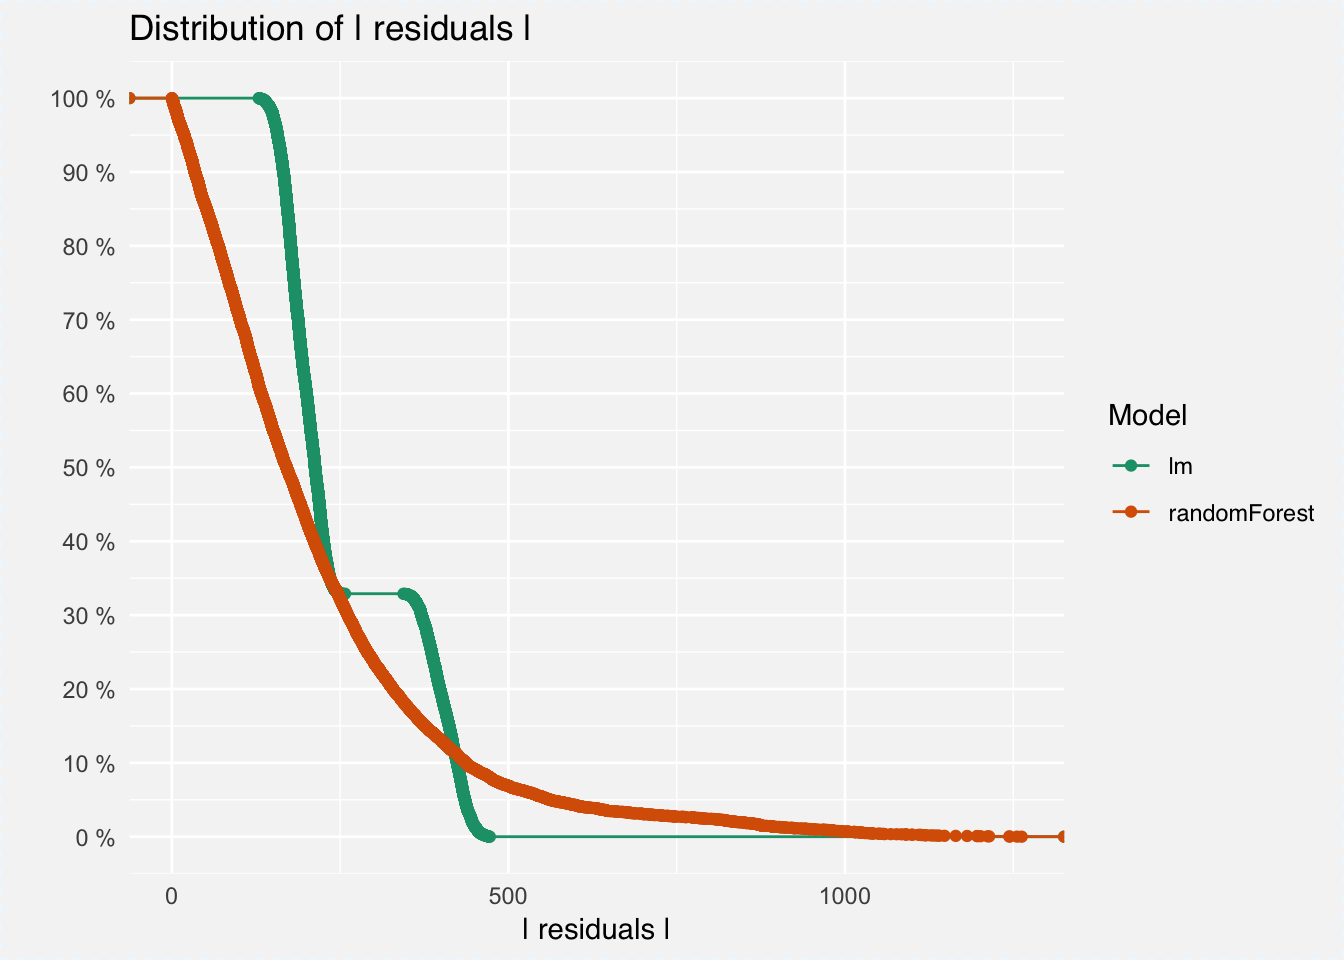
\includegraphics{DALEX_files/figure-latex/global_explain_ecdf-1.pdf}
\caption{(\#fig:global\_explain\_ecdf)Comparison of residuals for linear
model and random forest}
\end{figure}

Use the \texttt{geom\ =\ "boxplot"} parameter for the generic
\texttt{plot()} function to get an alternative comparison of residuals.
The red dot stands for the root mean square.

\begin{Shaded}
\begin{Highlighting}[]
\KeywordTok{plot}\NormalTok{(mp_lm, mp_rf, }\DataTypeTok{geom =} \StringTok{"boxplot"}\NormalTok{)}
\end{Highlighting}
\end{Shaded}

\begin{figure}
\centering
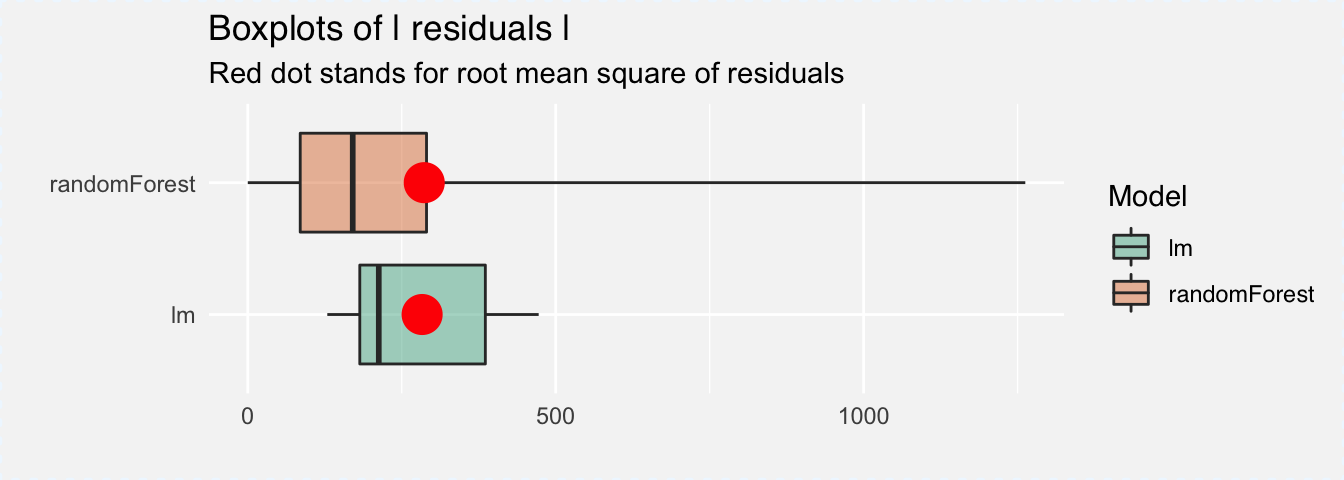
\includegraphics{DALEX_files/figure-latex/global_explain_boxplot-1.pdf}
\caption{(\#fig:global\_explain\_boxplot)Comparison of residuals for
linear model and random forest}
\end{figure}

\hypertarget{featureImportance}{%
\section{Feature importance}\label{featureImportance}}

Explainers presented in this section are designed to better understand
which variables are important.

Some models, such as linear regression or random forest, have a build-in
\emph{model specific} methods to calculate and visualize variable
importance. They will be presented in Section \ref{modelSpecific}.

Section \ref{modelAgnostic} presents a model agnostic approach on the
basis of permutations. The advantage of this approach is that different
models can be compared within a single setup.

\hypertarget{modelAgnostic}{%
\subsection{Model agnostic}\label{modelAgnostic}}

Model agnostic variable importance is calculated by means of
permutations. We simply substract the loss function calculated for
validation dataset with permuted values for a single variable from the
loss function calculated for validation dataset. This concept and some
extensions are described in \citep{variableImportancePermutations}.

This method is implemented in the \texttt{variable\_importance()}
function. The loss function is calculated for:

\begin{itemize}
\tightlist
\item
  the original validation \texttt{data}. It is an estimate of a model
  performance and will be denoted as \texttt{\_full\_model\_},
\item
  validation data with resampled \texttt{y} labels. It is a kind of
  \emph{worst case} loss when model are compared against random labels.
  It will be denoted as \texttt{\_baseline\_},
\item
  validation data with single variable being resampled. It tells us how
  much is gone from the model performance after the selected variable is
  blinded.
\end{itemize}

Let's see how this function works for a random forest model.

\begin{Shaded}
\begin{Highlighting}[]
\NormalTok{vi_rf <-}\StringTok{ }\KeywordTok{variable_importance}\NormalTok{(explainer_rf, }\DataTypeTok{loss_function =}\NormalTok{ loss_root_mean_square)}
\NormalTok{vi_rf}
\end{Highlighting}
\end{Shaded}

\begin{verbatim}
##            variable dropout_loss        label
## 1      _full_model_     285.1355 randomForest
## 2          no.rooms     391.0710 randomForest
## 3 construction.year     410.5866 randomForest
## 4             floor     445.2164 randomForest
## 5           surface     480.1431 randomForest
## 6          district     843.6519 randomForest
## 7        _baseline_    1081.3710 randomForest
\end{verbatim}

{Here the \texttt{loss\_root\_mean\_square()} function is defined as
square root from averaged squared differences between labels and model
predictions. } The same method may be applied to a linear model. Since
we are using the same loss function and the same method for variable
permutations, the losses calculated with both methods can be directly
compared.

\begin{Shaded}
\begin{Highlighting}[]
\NormalTok{vi_lm <-}\StringTok{ }\KeywordTok{variable_importance}\NormalTok{(explainer_lm, }\DataTypeTok{loss_function =}\NormalTok{ loss_root_mean_square)}
\NormalTok{vi_lm}
\end{Highlighting}
\end{Shaded}

\begin{verbatim}
##            variable dropout_loss label
## 1      _full_model_     284.2788    lm
## 2 construction.year     284.2638    lm
## 3          no.rooms     295.5020    lm
## 4             floor     495.7685    lm
## 5           surface     600.4308    lm
## 6          district    1025.7208    lm
## 7        _baseline_    1232.6798    lm
\end{verbatim}

It is much easier to compare both models when these values are plotted
close to each other. The generic \texttt{plot()} function may handle
both models.

\begin{Shaded}
\begin{Highlighting}[]
\KeywordTok{plot}\NormalTok{(vi_lm, vi_rf)}
\end{Highlighting}
\end{Shaded}

\begin{figure}
\centering
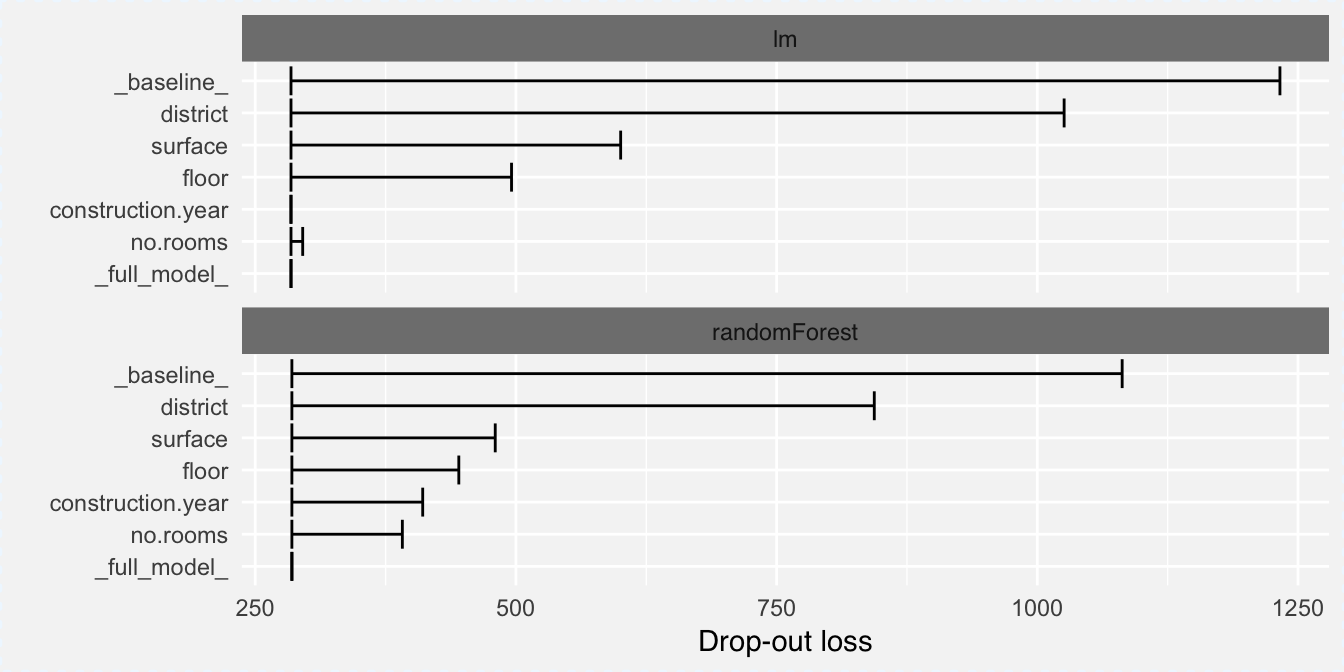
\includegraphics{DALEX_files/figure-latex/modelImportanceRaw-1.pdf}
\caption{\label{fig:modelImportanceRaw}Model agnostic variable importance
plot. Right edges correspond to loss function after permutation of a
single variable. Left edges correspond to loss of a full model}
\end{figure}

What we can read out of this plot?

\begin{itemize}
\tightlist
\item
  left edges of intervals start in \texttt{\_full\_model\_} for a given
  model. As we can see. the performances are similar for both models,
\item
  length of the interval corresponds to variable importance. In both
  models the most important variables are \texttt{district} and
  \texttt{surface},
\item
  in the random forest model the \texttt{construction\_year} variable
  has some importance, while its importance for linear model is almost
  equal to zero,
\item
  the variable \texttt{no.rooms} (which is correlated with
  \texttt{surface}) has some importance in the random forest model but
  not in the linear model.
\end{itemize}

We may be interested in variables that behave differently between models
(like \texttt{construction\_year}) or variables that are important in
both models (like \texttt{district} or \texttt{surface}). In the next
section we introduce explainers for further investigation of these
variables.

\emph{NOTE:} If you want variable importance hooked at 0, just add
\texttt{type\ =\ "difference"} parameter to
\texttt{variable\_importance()}.

\begin{Shaded}
\begin{Highlighting}[]
\NormalTok{vi_lm <-}\StringTok{ }\KeywordTok{variable_importance}\NormalTok{(explainer_lm, }\DataTypeTok{loss_function =}\NormalTok{ loss_root_mean_square, }\DataTypeTok{type =} \StringTok{"difference"}\NormalTok{)}
\NormalTok{vi_rf <-}\StringTok{ }\KeywordTok{variable_importance}\NormalTok{(explainer_rf, }\DataTypeTok{loss_function =}\NormalTok{ loss_root_mean_square, }\DataTypeTok{type =} \StringTok{"difference"}\NormalTok{)}
\KeywordTok{plot}\NormalTok{(vi_lm, vi_rf)}
\end{Highlighting}
\end{Shaded}

\begin{figure}
\centering
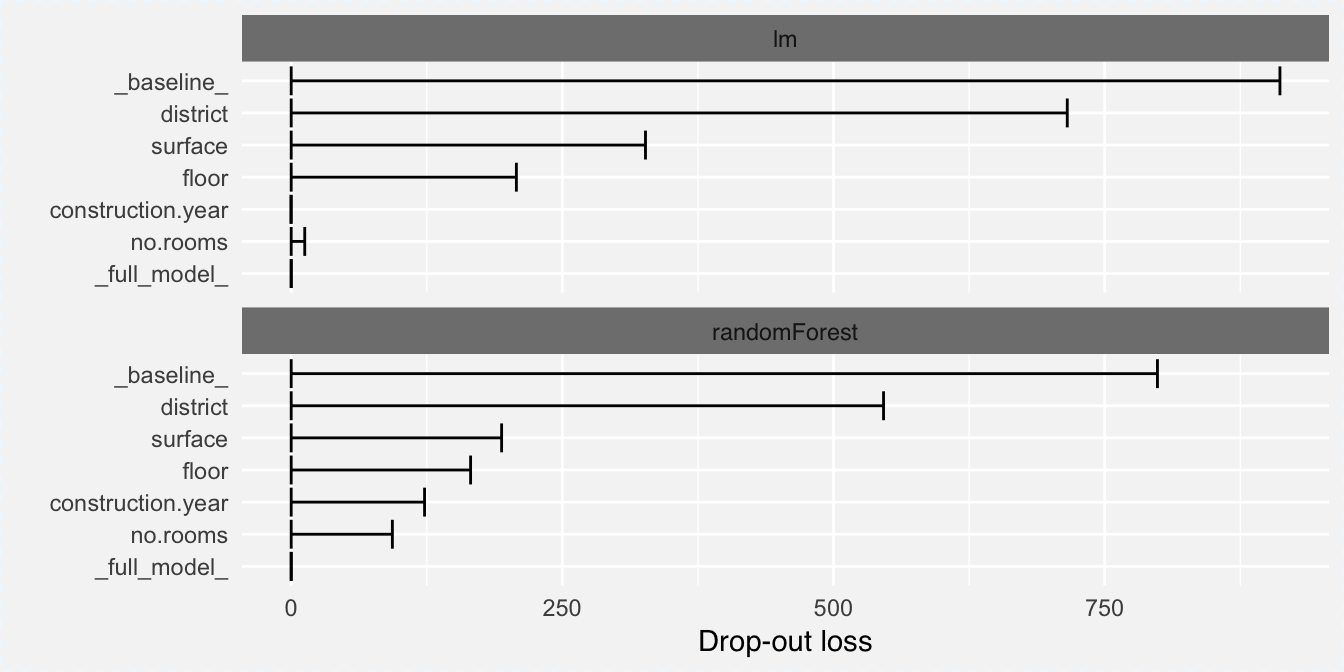
\includegraphics{DALEX_files/figure-latex/modelImportanceDifference-1.pdf}
\caption{\label{fig:modelImportanceDifference}Model agnostic variable
importance plot. Right edges correspond to difference between loss after
permutation of a single variable and loss of a full model}
\end{figure}

\hypertarget{modelSpecific}{%
\subsection{Model specific}\label{modelSpecific}}

Some models have build-in tools for calculation of variable importance.
Random forest uses two different measures - one based on out-of-bag data
and second one based on gains in nodes. Read more about this approach in
\citep{randomForest}.

Below we show an example of a dot plot that summarizes default
importance measure for a random forest. The \texttt{varImpPlot()}
function is available in the \texttt{randomForest} package.

\begin{Shaded}
\begin{Highlighting}[]
\KeywordTok{varImpPlot}\NormalTok{(apartments_rf_model)}
\end{Highlighting}
\end{Shaded}

\begin{figure}
\centering
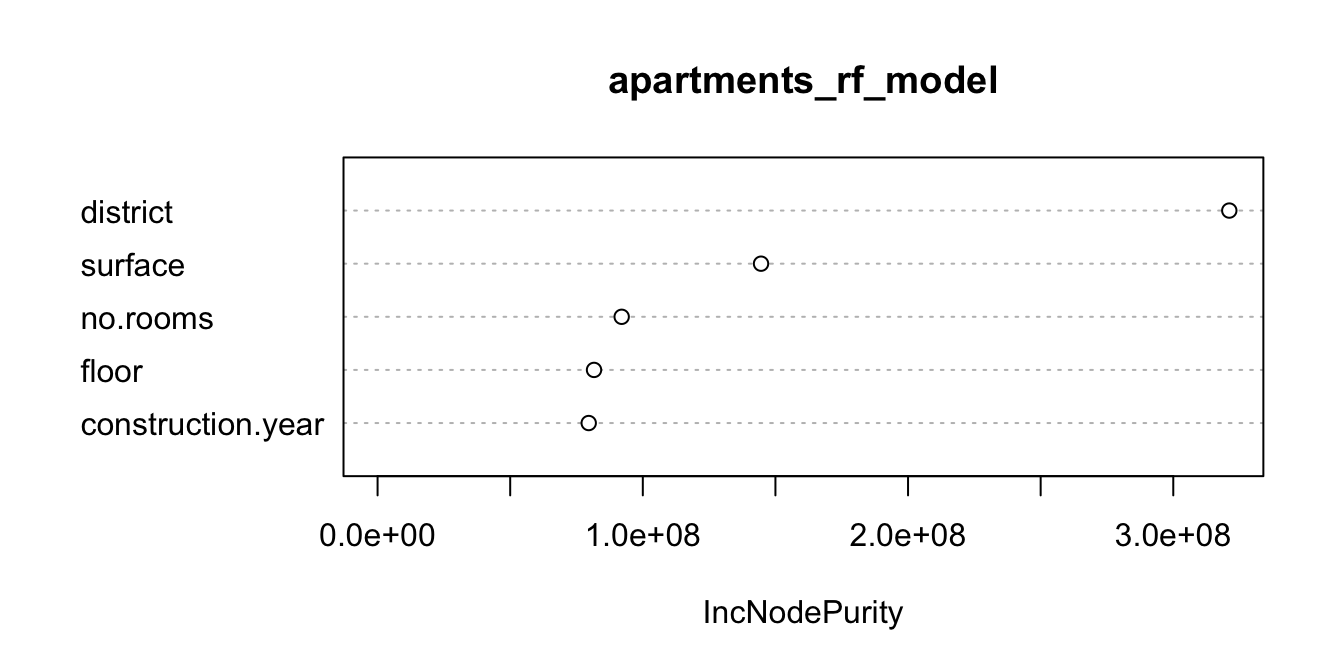
\includegraphics{DALEX_files/figure-latex/modelImportanceRF-1.pdf}
\caption{\label{fig:modelImportanceRF}Built-in variable importance plot for
random forest}
\end{figure}

It is easy to assess variable importance for linear models and
generalized models, since model coefficients have direct interpretation.

\href{https://en.wikipedia.org/wiki/Forest_plot}{Forest plots} were
initially used in the meta analysis to visualize effects in different
studies. . At present, however, they are frequently used to present
summary characteristics for models with linear structure / created with
\texttt{lm} or \texttt{glm} functions.

There are various implementations of forest plots in R. In the package
\texttt{forestmodel} (see \citep{forestmodel}) one can use
\texttt{forest\_model()} function to draw a forest plot. This package is
based on the \texttt{broom} package (see \citep{broom}) and this is why
it handles a large variety of different regression models.

\begin{Shaded}
\begin{Highlighting}[]
\KeywordTok{library}\NormalTok{(}\StringTok{"forestmodel"}\NormalTok{)}
\KeywordTok{forest_model}\NormalTok{(apartments_lm_model)}
\end{Highlighting}
\end{Shaded}

\begin{figure}
\centering
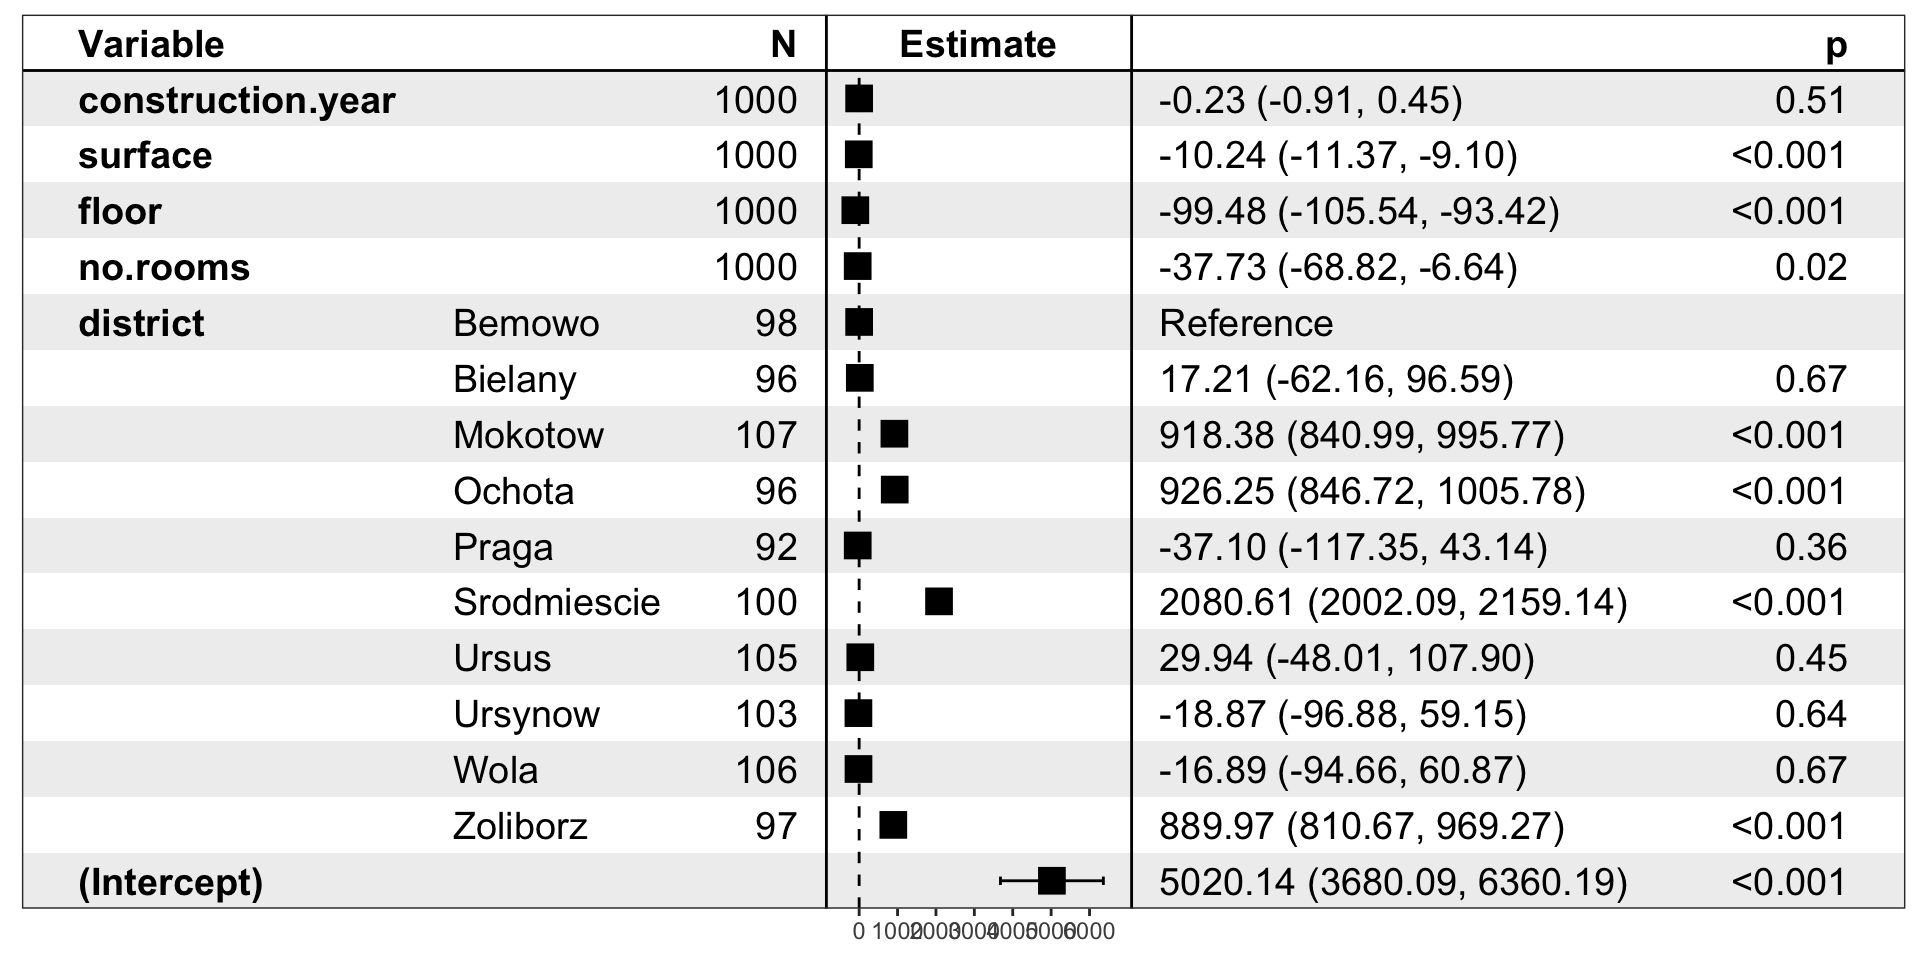
\includegraphics{DALEX_files/figure-latex/forestmodel-1.pdf}
\caption{\label{fig:forestmodel}Forest plot created with
\texttt{forestmodel} package}
\end{figure}

In the package \texttt{sjPlot} (see \citep{sjPlot}) one can find
\texttt{sjp.xyz()} function to visualize coefficients of a \texttt{xyz}
model (like \texttt{sjp.glm()} for \texttt{glm} models) or a generic
wrapper \texttt{plot\_model()}.

\begin{Shaded}
\begin{Highlighting}[]
\KeywordTok{library}\NormalTok{(}\StringTok{"sjPlot"}\NormalTok{)}
\KeywordTok{plot_model}\NormalTok{(apartments_lm_model, }\DataTypeTok{type =} \StringTok{"est"}\NormalTok{, }\DataTypeTok{sort.est =} \OtherTok{TRUE}\NormalTok{)}
\end{Highlighting}
\end{Shaded}

\begin{figure}
\centering
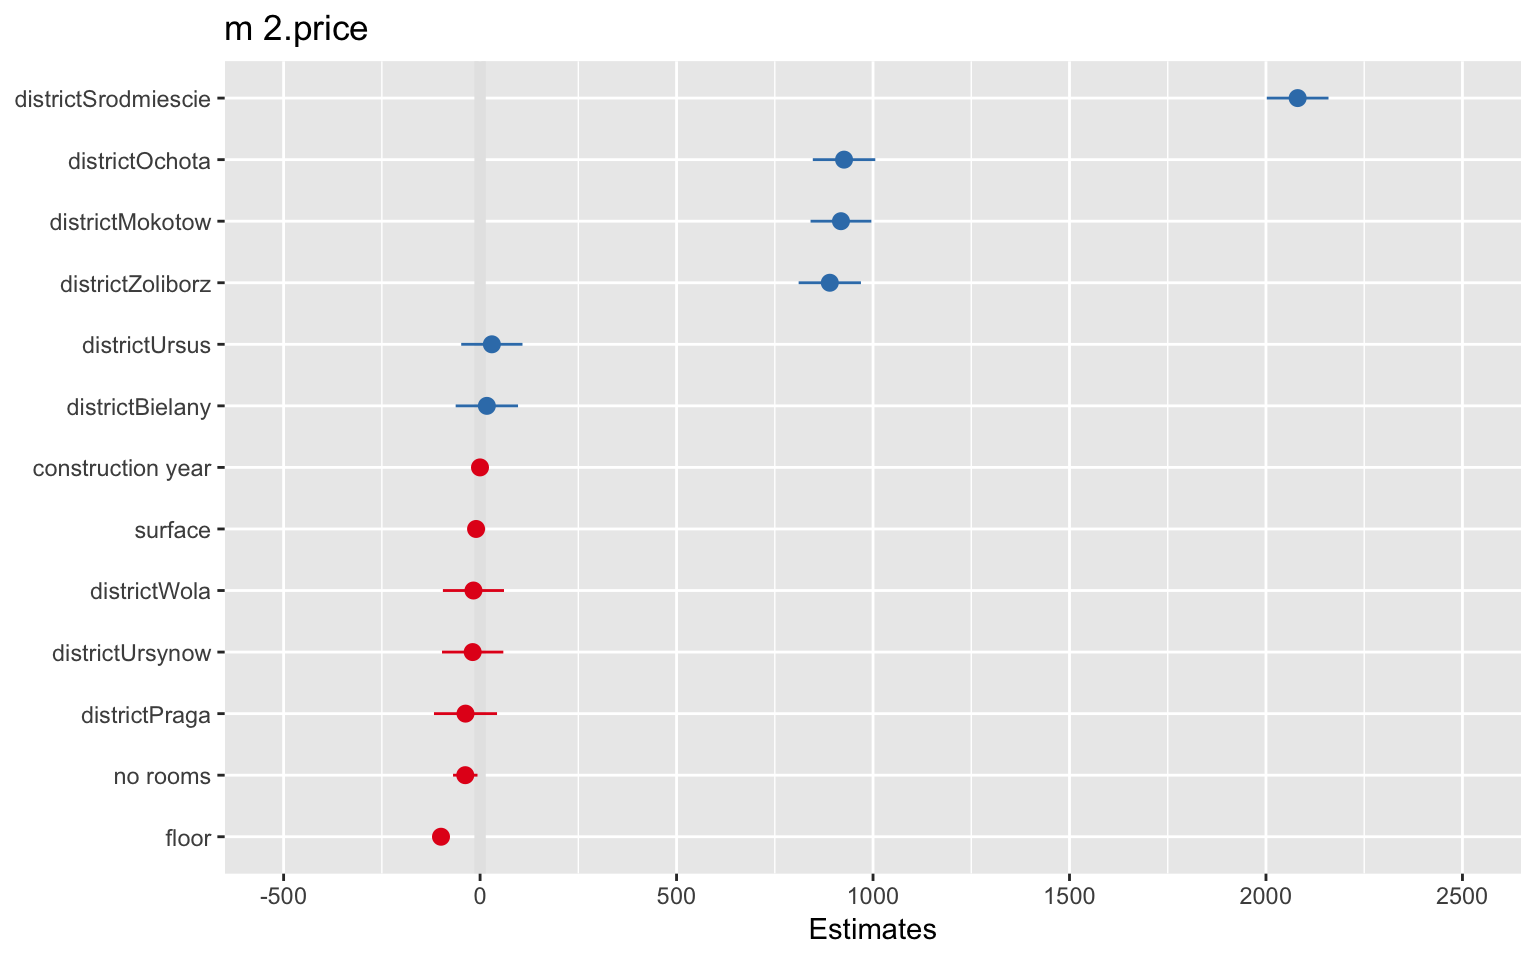
\includegraphics{DALEX_files/figure-latex/sjpglm-1.pdf}
\caption{\label{fig:sjpglm}Model coefficients plotted with sjPlot package}
\end{figure}

\textbf{Note!}

The \texttt{forestmodel} package handles factor variables in a better
way while the plots from \texttt{sjPlot} are easier to read.

\hypertarget{variableResponse}{%
\section{Variable response}\label{variableResponse}}

Explainers presented in this section are designed to better understand
the relation between a variable and a model output.

Subsection \ref{pdpchapter} presents Partial Dependence Plots (PDP), one
of the most popular methods for exploration of a relation between a
continuous variable and a model outcome. Subsection
\ref{accumulatedLocalEffects} presents Accumulated Local Effects Plots
(ALEP), an extension of PDP more suited for highly correlated variables.

Subsection \ref{mergingPathPlot} presents Merging Path Plots, a method
for exploration of a relation between a categorical variable and a model
outcome.

\hypertarget{pdpchapter}{%
\subsection{Partial Dependence Plot}\label{pdpchapter}}

Partial Dependence Plots (see \texttt{pdp} package \citep{pdp}) for a
black box \(f(x; \theta)\) show the expected output condition on a
selected variable.

\[
p_i(x_i) = E_{x_{-i}}[ f(x^i, x^{-i}; \theta) ].
\]

Of course, this expectation cannot be calculated directly as we do not
know fully neither the distribution of \(x_{-i}\) nor the \(f()\). Yet
this value may be estimated by

\[
\hat p_i(x_i) = \frac{1}{n} \sum_{j=1}^{n} f(x^i_j, x_j^{-i}, \hat \theta).
\]

Let's see an example for the model \texttt{apartments\_rf\_model}. Below
we use \texttt{variable\_response()} from \texttt{DALEX}, which calls
\texttt{pdp::partial} function to calculate PDP response.

Section \ref{featureImportance} shows variable importance plots for
different models. The variable \texttt{construction.year} is interesting
as it is important for the random forest model
\texttt{apartments\_rf\_model} but not for the linear model
\texttt{apartments\_lm\_model}. Let's see the relation between the
variable and the model output.

\begin{Shaded}
\begin{Highlighting}[]
\NormalTok{sv_rf  <-}\StringTok{ }\KeywordTok{single_variable}\NormalTok{(explainer_rf, }\DataTypeTok{variable =}  \StringTok{"construction.year"}\NormalTok{, }\DataTypeTok{type =} \StringTok{"pdp"}\NormalTok{)}
\KeywordTok{plot}\NormalTok{(sv_rf)}
\end{Highlighting}
\end{Shaded}

\begin{figure}
\centering
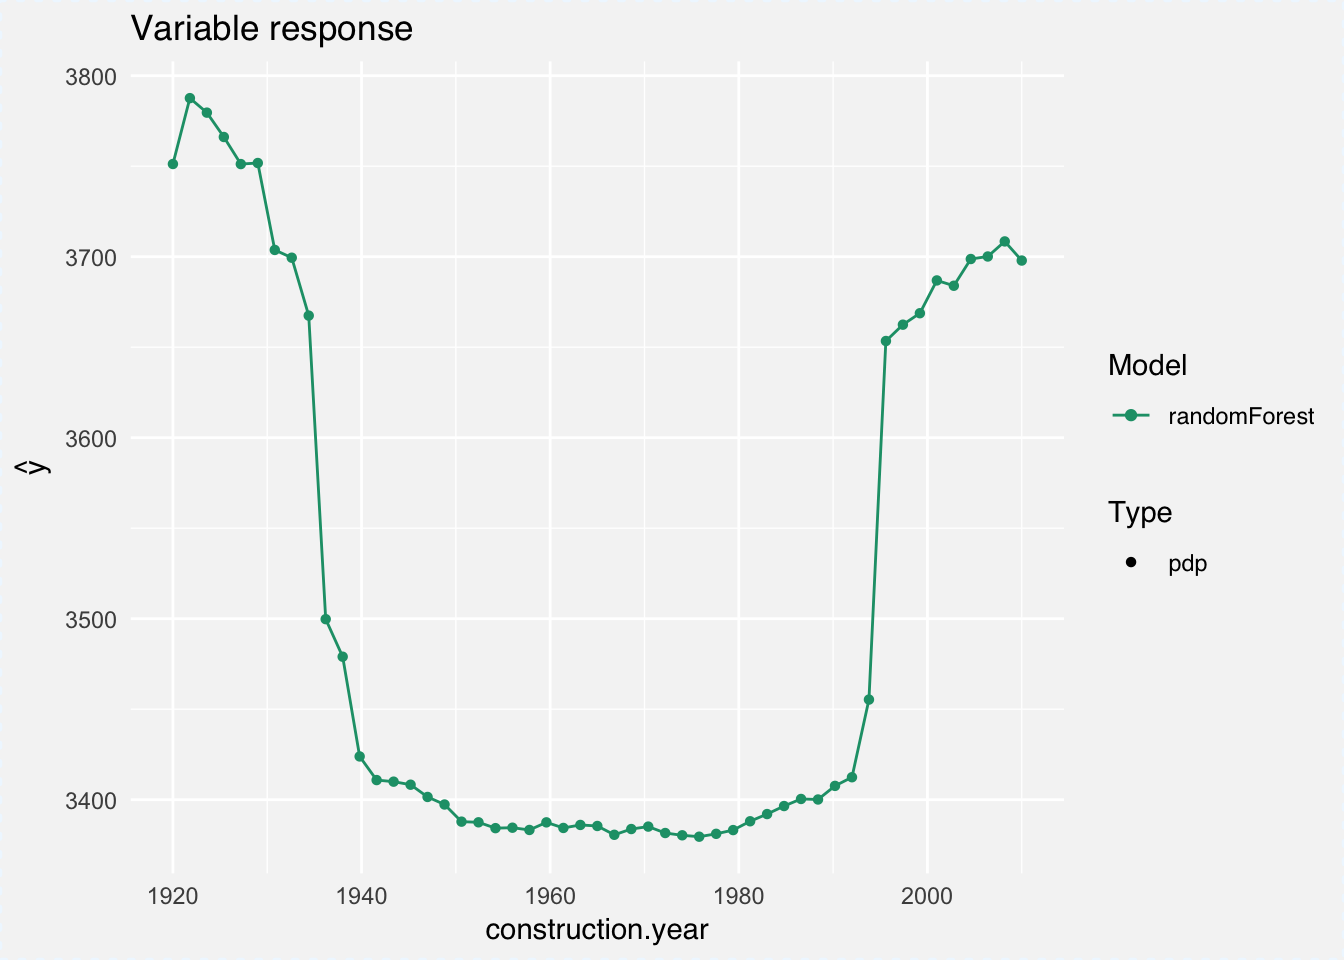
\includegraphics{DALEX_files/figure-latex/pdpRandomForest-1.pdf}
\caption{\label{fig:pdpRandomForest}Relation between output from
\texttt{apartments\_rf\_model} and variable \texttt{construction.year}}
\end{figure}

We can use PDP plots to compare two or more models. Below we plot PDP
for the linear model against the random forest model.

\begin{Shaded}
\begin{Highlighting}[]
\NormalTok{sv_lm  <-}\StringTok{ }\KeywordTok{single_variable}\NormalTok{(explainer_lm, }\DataTypeTok{variable =}  \StringTok{"construction.year"}\NormalTok{, }\DataTypeTok{type =} \StringTok{"pdp"}\NormalTok{)}

\KeywordTok{plot}\NormalTok{(sv_rf, sv_lm)}
\end{Highlighting}
\end{Shaded}

\begin{figure}
\centering
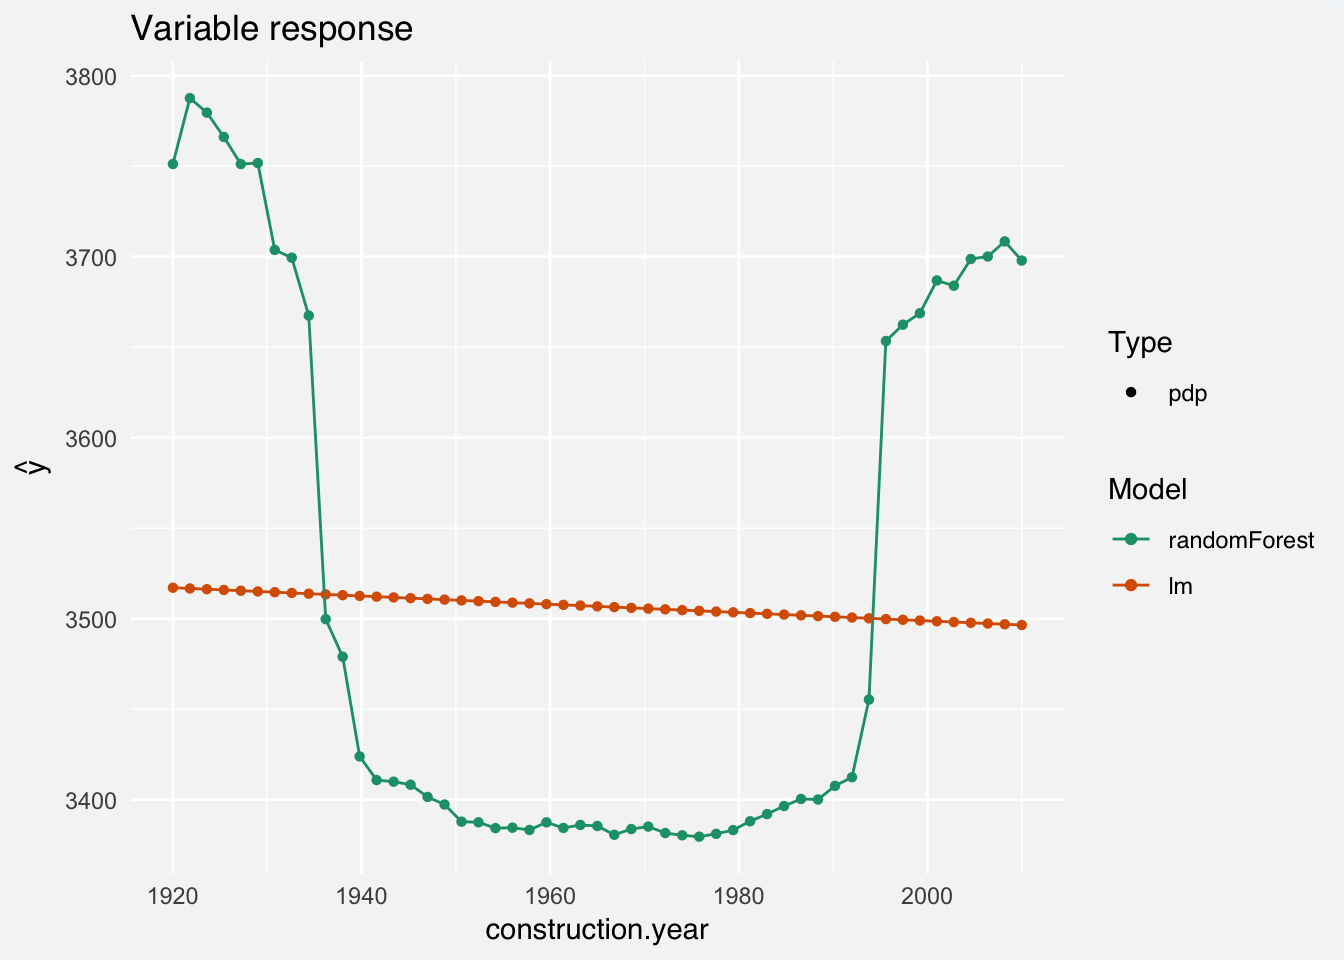
\includegraphics{DALEX_files/figure-latex/pdpRandomForestLM-1.pdf}
\caption{\label{fig:pdpRandomForestLM}Relation between output from models
\texttt{apartments\_rf\_model} and \texttt{apartments\_lm\_model}
against the variable \texttt{construction.year}}
\end{figure}

It looks like the random forest captures the non-linear relation that
cannot be captured by linear models.

\hypertarget{accumulatedLocalEffects}{%
\subsection{Accumulated Local Effects
Plot}\label{accumulatedLocalEffects}}

As demonstrated in section \ref{pdpchapter}, the Partial Dependence Plot
presents the expected model response with respect to marginal
distribution of \(x_{-i}\). In some cases, e.g.~when repressors are
highly correlated, expectation towards the marginal distribution may
lead to biases/poorly extrapolated model responses.

Accumulated local effects (ALE) plots (see \texttt{ALEPlot} package
\citep{ALEPlot}) solve this problem by using conditional distribution
\(x_{-i}|x_i = x_i^*\). This solution leads to more stable and reliable
estimates (at least when the predictors are highly correlated).

Estimation of the main effects for \texttt{construction.year} is similar
to the PDP curves. We use here \texttt{DALEX::single\_variable} function
that calls \texttt{ALEPlot::ALEPlot} function to calculate the ALE curve
for the variable \texttt{construction.year}.

\begin{Shaded}
\begin{Highlighting}[]
\NormalTok{sva_rf  <-}\StringTok{ }\KeywordTok{single_variable}\NormalTok{(explainer_rf, }\DataTypeTok{variable =} \StringTok{"construction.year"}\NormalTok{, }\DataTypeTok{type =} \StringTok{"ale"}\NormalTok{)}
\NormalTok{sva_lm  <-}\StringTok{ }\KeywordTok{single_variable}\NormalTok{(explainer_lm, }\DataTypeTok{variable =} \StringTok{"construction.year"}\NormalTok{, }\DataTypeTok{type =} \StringTok{"ale"}\NormalTok{)}
\end{Highlighting}
\end{Shaded}

\begin{figure}
\centering
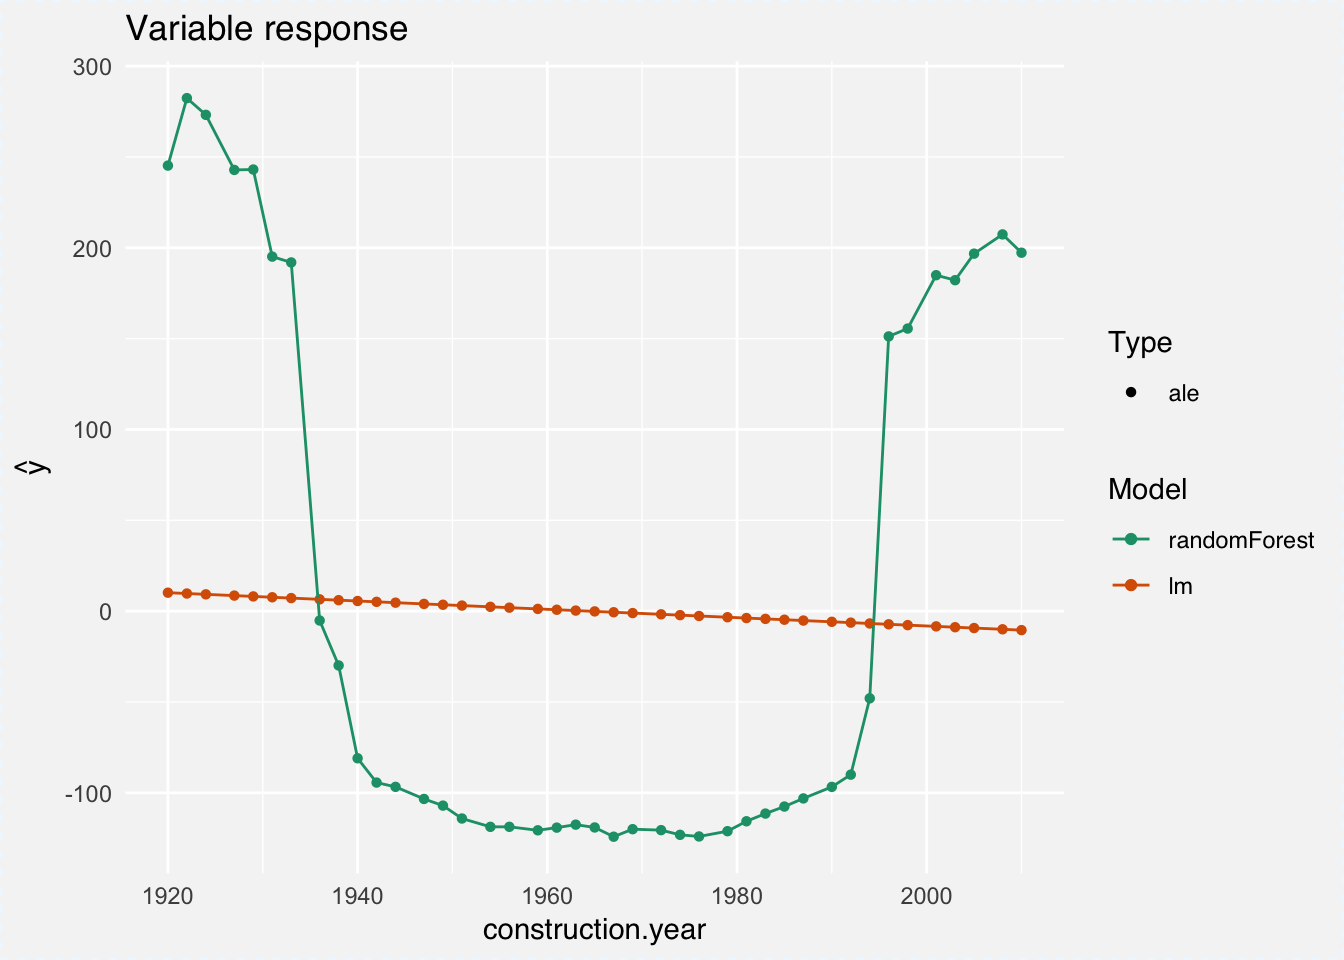
\includegraphics{DALEX_files/figure-latex/alePlotsRF-1.pdf}
\caption{\label{fig:alePlotsRF}Relation between output from models
\texttt{apartments\_rf\_model} and \texttt{apartments\_lm\_model}
against the variable \texttt{construction.year} calculated with
Accumulated local effects.}
\end{figure}

\begin{Shaded}
\begin{Highlighting}[]
\KeywordTok{plot}\NormalTok{(sva_rf, sva_lm)}
\end{Highlighting}
\end{Shaded}

\begin{figure}
\centering
\includegraphics{DALEX_files/figure-latex/alePlotsRF-2.pdf}
\caption{\label{fig:alePlotsRF}Relation between output from models
\texttt{apartments\_rf\_model} and \texttt{apartments\_lm\_model}
against the variable \texttt{construction.year} calculated with
Accumulated local effects.}
\end{figure}

Results for PDP and ALEP are very similar except that effects for ALEP
are centered around 0.

\hypertarget{mergingPathPlot}{%
\subsection{Mering Path Plot}\label{mergingPathPlot}}

The package \texttt{ICEbox} does not work for factor variables, while
the \texttt{pdp} package returns plots that are hard to interpret.

An interesting tool that helps to understand what happens with factor
variables is the \textbf{factorMerger} package. See
\citep{factorMerger}.

Below you may see a Merging Path Plot for a factor variable
\texttt{district}.

\begin{Shaded}
\begin{Highlighting}[]
\NormalTok{svd_rf  <-}\StringTok{ }\KeywordTok{single_variable}\NormalTok{(explainer_rf, }\DataTypeTok{variable =} \StringTok{"district"}\NormalTok{, }\DataTypeTok{type =} \StringTok{"factor"}\NormalTok{)}
\NormalTok{svd_lm  <-}\StringTok{ }\KeywordTok{single_variable}\NormalTok{(explainer_lm, }\DataTypeTok{variable =} \StringTok{"district"}\NormalTok{, }\DataTypeTok{type =} \StringTok{"factor"}\NormalTok{)}

\KeywordTok{plot}\NormalTok{(svd_rf, svd_lm)}
\end{Highlighting}
\end{Shaded}

\begin{figure}
\centering
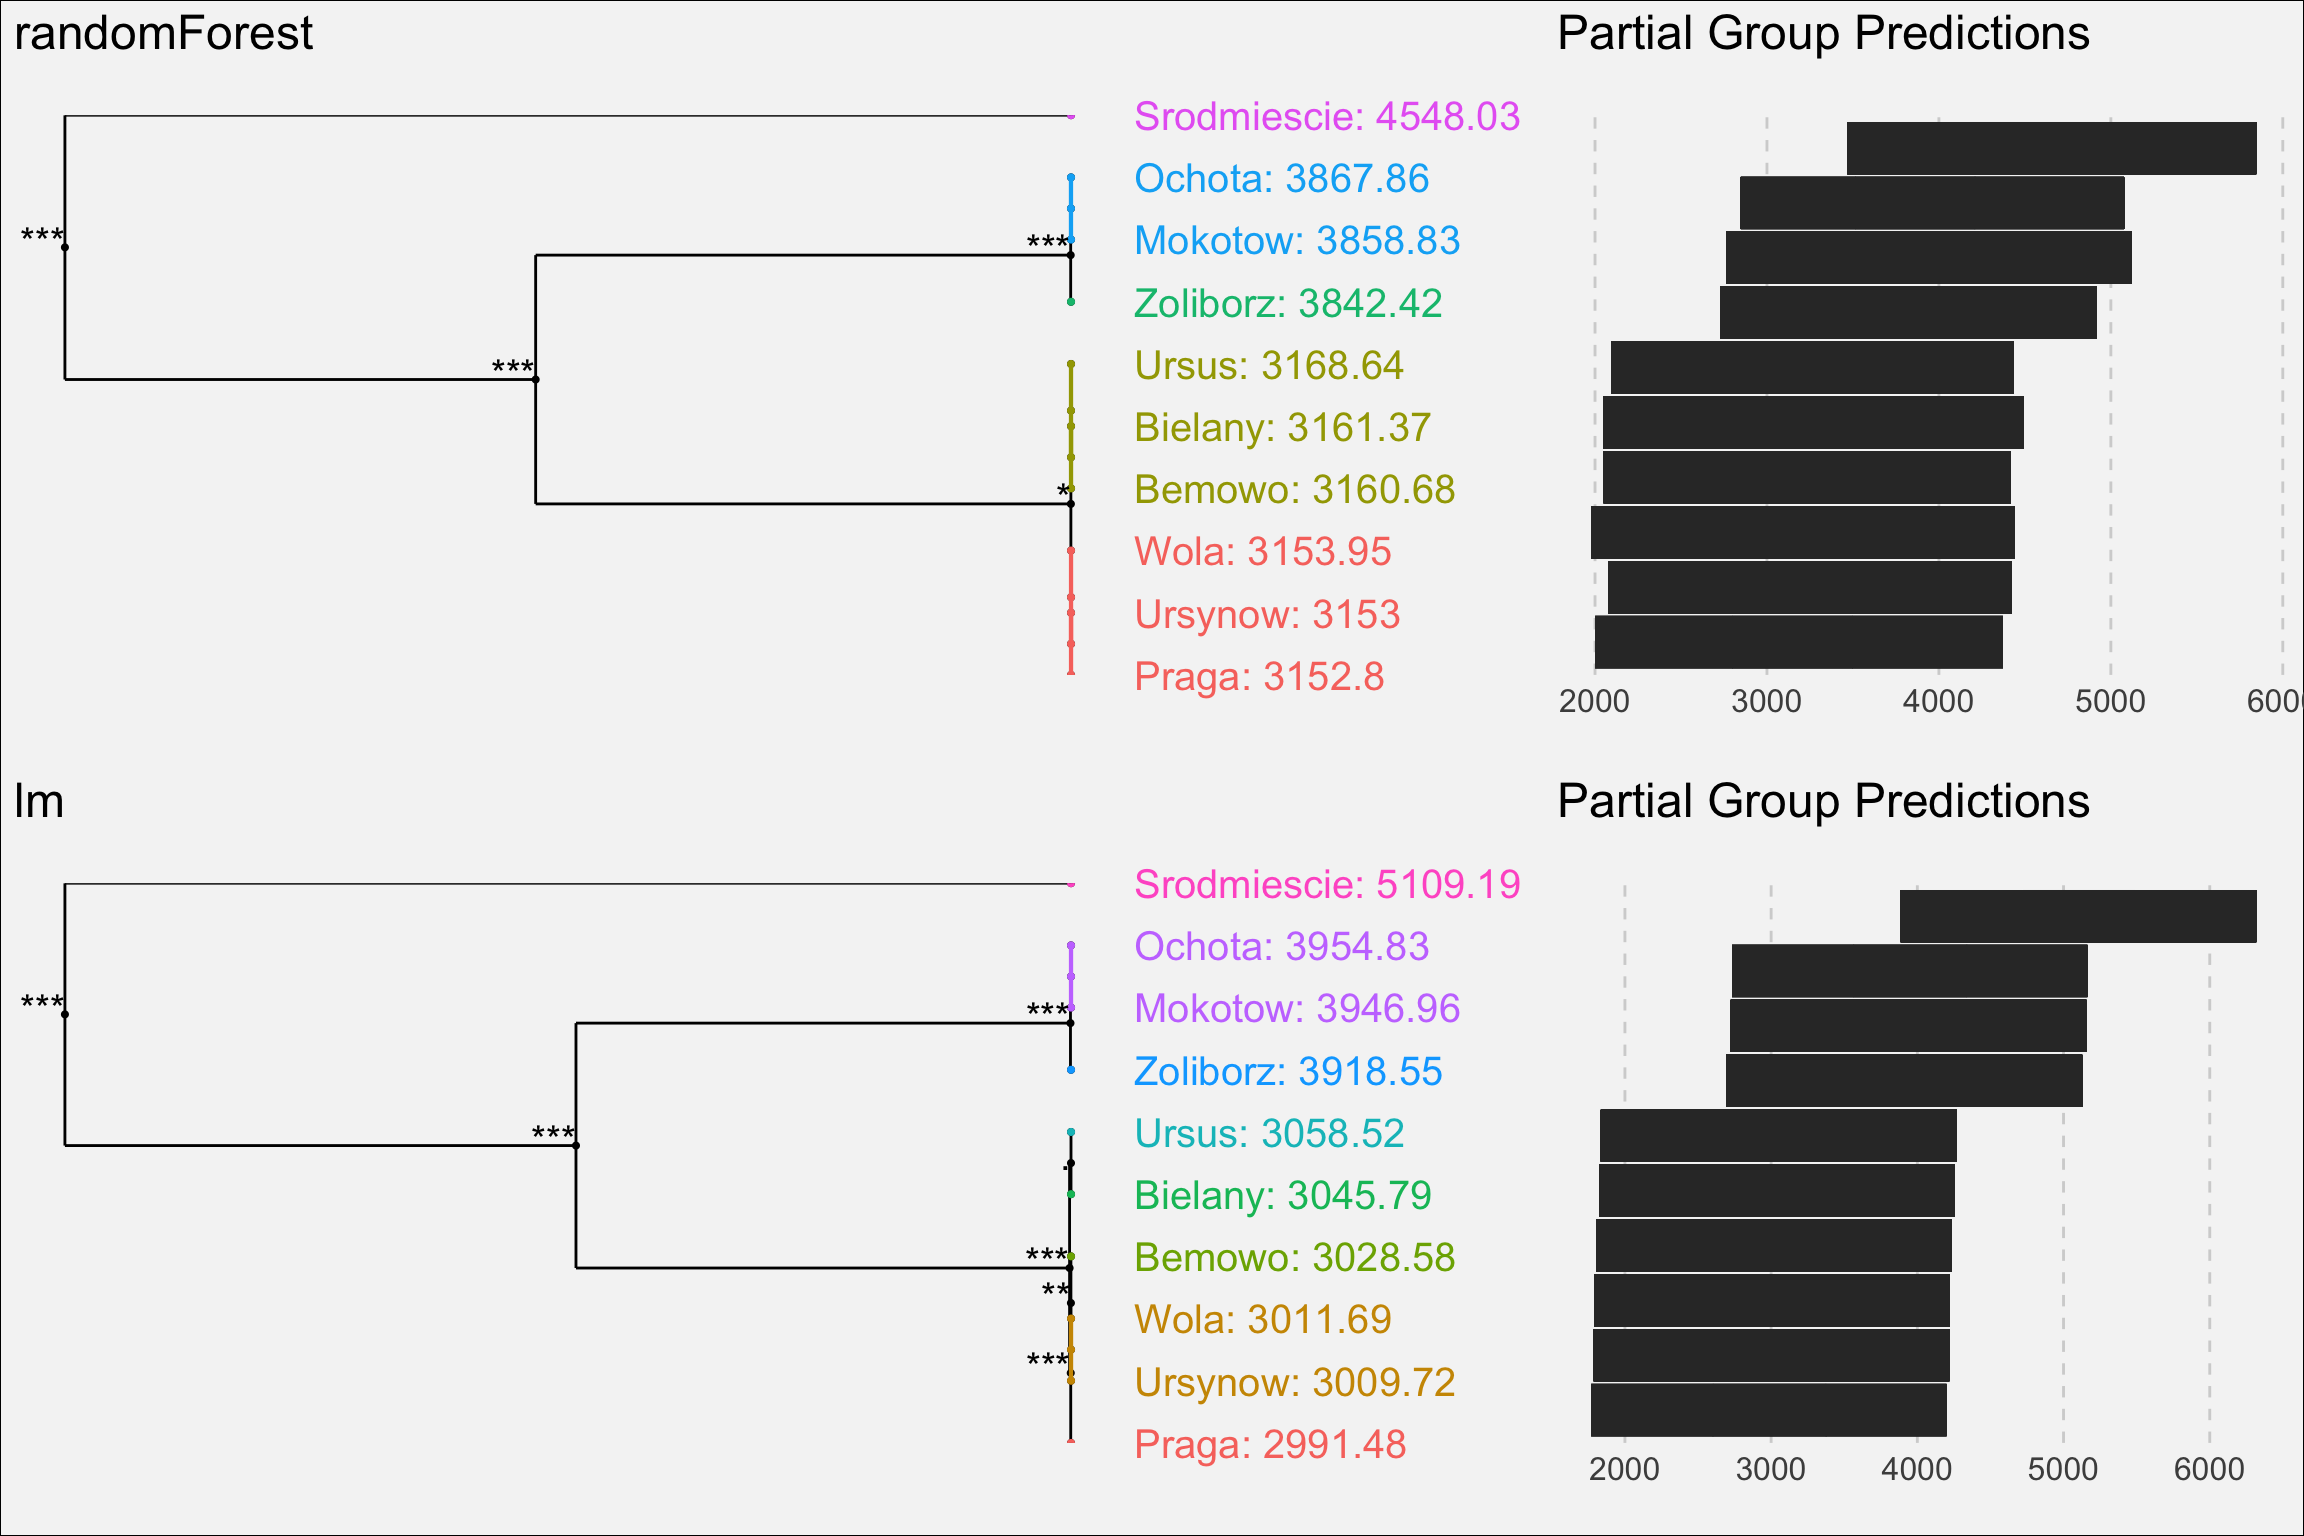
\includegraphics{DALEX_files/figure-latex/mergingPathPlots-1.pdf}
\caption{\label{fig:mergingPathPlots}Merging Path Plot for \texttt{district}
variable. Left panel shows the dendrogram for districts, here we have
clearly three clusters. Right panel shows distribution of predictions
for each district.}
\end{figure}

The three clusters are: the city center (Srodmiescie), districts well
communicated with city center (Ochota, Mokotow, Zoliborz) and other
districts closer to city boundaries.

Factor variables are handled very differently by random forest and
linear model, yet despite these differences both models result in very
similar plots.

\hypertarget{predictionUnderstanding}{%
\chapter{Prediction understanding}\label{predictionUnderstanding}}

In this chapter we introduce two groups of explainers that can be used
to boost our understanding of model predictions.

\begin{itemize}
\tightlist
\item
  Section \ref{outlierDetection} presents explainers that helps to
  identify outliers.
\item
  Section \ref{predictionBreakdown} presents explainers for model
  predictions. Each prediction can be split into parts attributed to
  particular variables. Having found out which variables are important
  and whether the prediction is accurate, one can validate the model.
\end{itemize}

Explainers presented here are illustrated based on two models fitted to
the \texttt{apartments} data.

\begin{Shaded}
\begin{Highlighting}[]
\KeywordTok{library}\NormalTok{(}\StringTok{"DALEX"}\NormalTok{)}
\NormalTok{apartments_lm_model <-}\StringTok{ }\KeywordTok{lm}\NormalTok{(m2.price }\OperatorTok{~}\StringTok{ }\NormalTok{construction.year }\OperatorTok{+}\StringTok{ }\NormalTok{surface }\OperatorTok{+}\StringTok{ }\NormalTok{floor }\OperatorTok{+}\StringTok{ }
\StringTok{                      }\NormalTok{no.rooms }\OperatorTok{+}\StringTok{ }\NormalTok{district, }\DataTypeTok{data =}\NormalTok{ apartments)}
\KeywordTok{library}\NormalTok{(}\StringTok{"randomForest"}\NormalTok{)}
\KeywordTok{set.seed}\NormalTok{(}\DecValTok{59}\NormalTok{)}
\NormalTok{apartments_rf_model <-}\StringTok{ }\KeywordTok{randomForest}\NormalTok{(m2.price }\OperatorTok{~}\StringTok{ }\NormalTok{construction.year }\OperatorTok{+}\StringTok{ }\NormalTok{surface }\OperatorTok{+}\StringTok{ }\NormalTok{floor }\OperatorTok{+}\StringTok{ }
\StringTok{                      }\NormalTok{no.rooms }\OperatorTok{+}\StringTok{ }\NormalTok{district, }\DataTypeTok{data =}\NormalTok{ apartments)}
\end{Highlighting}
\end{Shaded}

First we need to prepare wrappers for these models. They are in
\texttt{explainer\_lm} and \texttt{explainer\_rf} objects.

\begin{Shaded}
\begin{Highlighting}[]
\NormalTok{explainer_lm <-}\StringTok{ }\KeywordTok{explain}\NormalTok{(apartments_lm_model, }
                       \DataTypeTok{data =}\NormalTok{ apartmentsTest[,}\DecValTok{2}\OperatorTok{:}\DecValTok{6}\NormalTok{], }\DataTypeTok{y =}\NormalTok{ apartmentsTest}\OperatorTok{$}\NormalTok{m2.price)}
\NormalTok{explainer_rf <-}\StringTok{ }\KeywordTok{explain}\NormalTok{(apartments_rf_model, }
                       \DataTypeTok{data =}\NormalTok{ apartmentsTest[,}\DecValTok{2}\OperatorTok{:}\DecValTok{6}\NormalTok{], }\DataTypeTok{y =}\NormalTok{ apartmentsTest}\OperatorTok{$}\NormalTok{m2.price)}
\end{Highlighting}
\end{Shaded}

\hypertarget{outlierDetection}{%
\section{Outlier detection}\label{outlierDetection}}

Function \texttt{model\_performance()} may be used to identify outliers.
This function was already introduced in section \ref{modelPerformance}
but we will present here its other uses.

As you may remember, residuals for random forest were smaller in
general, except for a small fraction of very high residuals.

Let's use the \texttt{model\_performance()} function to extract and plot
residuals against the observed true values.

\begin{Shaded}
\begin{Highlighting}[]
\NormalTok{mp_rf <-}\StringTok{ }\KeywordTok{model_performance}\NormalTok{(explainer_rf)}

\KeywordTok{library}\NormalTok{(}\StringTok{"ggplot2"}\NormalTok{)}
\KeywordTok{ggplot}\NormalTok{(mp_rf, }\KeywordTok{aes}\NormalTok{(observed, diff)) }\OperatorTok{+}\StringTok{ }\KeywordTok{geom_point}\NormalTok{() }\OperatorTok{+}\StringTok{ }
\StringTok{        }\KeywordTok{xlab}\NormalTok{(}\StringTok{"Observed"}\NormalTok{) }\OperatorTok{+}\StringTok{ }\KeywordTok{ylab}\NormalTok{(}\StringTok{"Predicted - Observed"}\NormalTok{) }\OperatorTok{+}\StringTok{ }
\StringTok{        }\KeywordTok{ggtitle}\NormalTok{(}\StringTok{"Diagnostic plot for the random forest model"}\NormalTok{) }\OperatorTok{+}\StringTok{ }\KeywordTok{theme_mi2}\NormalTok{()}
\end{Highlighting}
\end{Shaded}

\begin{figure}
\centering
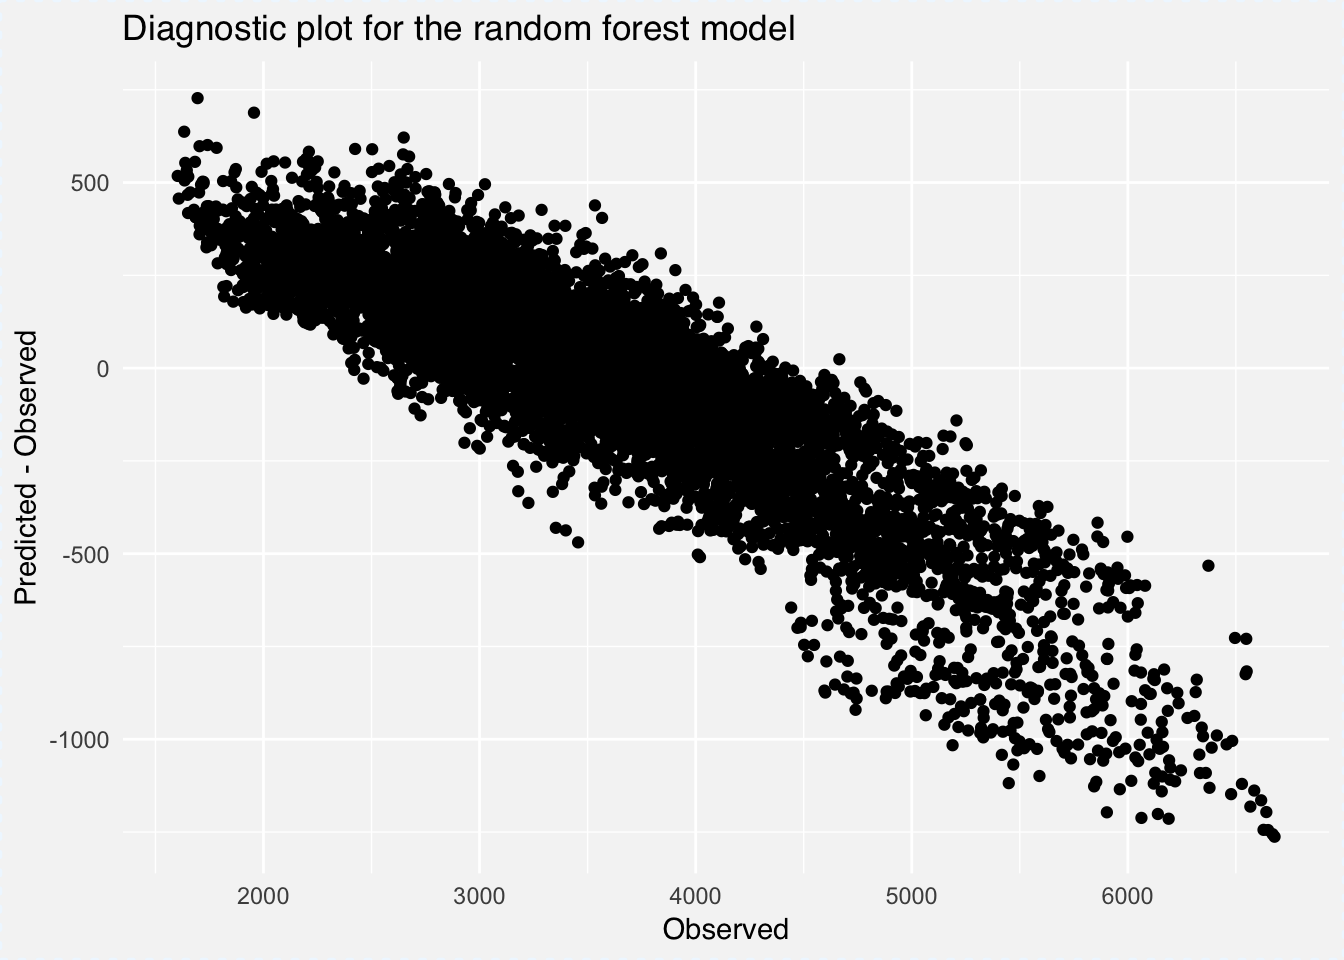
\includegraphics{DALEX_files/figure-latex/outliersML-1.pdf}
\caption{\label{fig:outliersML}Diagnostic plot for the random forest model.
Clearly the more expensive are apartments the more underestimated are
model predictions}
\end{figure}

Lets see which variables stand behind the model prediction for an
apartment with largest residual.

\begin{Shaded}
\begin{Highlighting}[]
\KeywordTok{which.min}\NormalTok{(mp_rf}\OperatorTok{$}\NormalTok{diff)}
\NormalTok{## 1161}
\NormalTok{new_apartment <-}\StringTok{ }\NormalTok{apartmentsTest[}\KeywordTok{which.min}\NormalTok{(mp_rf}\OperatorTok{$}\NormalTok{diff), ]}
\NormalTok{new_apartment}
\end{Highlighting}
\end{Shaded}

\begin{table}

\caption{\label{tab:unnamed-chunk-21}Observation with the largest residual in the random forest model}
\centering
\begin{tabular}[t]{l|r|r|r|r|r|l}
\hline
  & m2.price & construction.year & surface & floor & no.rooms & district\\
\hline
1161 & 6679 & 2005 & 22 & 1 & 2 & Srodmiescie\\
\hline
\end{tabular}
\end{table}

\hypertarget{predictionBreakdown}{%
\section{Prediction breakDown}\label{predictionBreakdown}}

Does your ML algorithm learn from mistakes? Understanding what causes
wrong model predictions will help to improve the model itself.

Lots of arguments in favor of such explainers can be found in the
\citep{lime} article. This approach is implemented in the \textbf{live}
package (see \citep{live}) which may be seen as an extension of the LIME
method.

In this section we present other method for explanations of model
predictions, namely the one implemented in the \texttt{breakDown}
package \citep{breakDown}. The function \texttt{single\_prediction()} is
a wrapper around this package.

Model prediction is visualized with Break Down Plots, which were
inspired by waterfall plots as in
\href{https://github.com/AppliedDataSciencePartners/xgboostExplainer}{\texttt{xgboostExplainer}
package}. Break Down Plots show the contribution of every variable
present in the model.

Function \texttt{single\_prediction()} generates variable attributions
for selected prediction. The generic \texttt{plot()} function shows
these attributions.

\begin{Shaded}
\begin{Highlighting}[]
\NormalTok{new_apartment_rf <-}\StringTok{ }\KeywordTok{single_prediction}\NormalTok{(explainer_rf, }\DataTypeTok{observation =}\NormalTok{ new_apartment)}
\NormalTok{breakDown}\OperatorTok{:::}\KeywordTok{print.broken}\NormalTok{(new_apartment_rf)}
\end{Highlighting}
\end{Shaded}

\begin{verbatim}
##                            contribution
## (Intercept)                       0.000
## + district = Srodmiescie       1042.059
## + surface = 22                  364.385
## + floor = 1                     279.526
## + no.rooms = 2                  279.070
## + construction.year = 2005      -54.566
## final_prognosis                1910.474
## baseline:  3505.971
\end{verbatim}

\begin{Shaded}
\begin{Highlighting}[]
\KeywordTok{plot}\NormalTok{(new_apartment_rf)}
\end{Highlighting}
\end{Shaded}

\begin{figure}
\centering
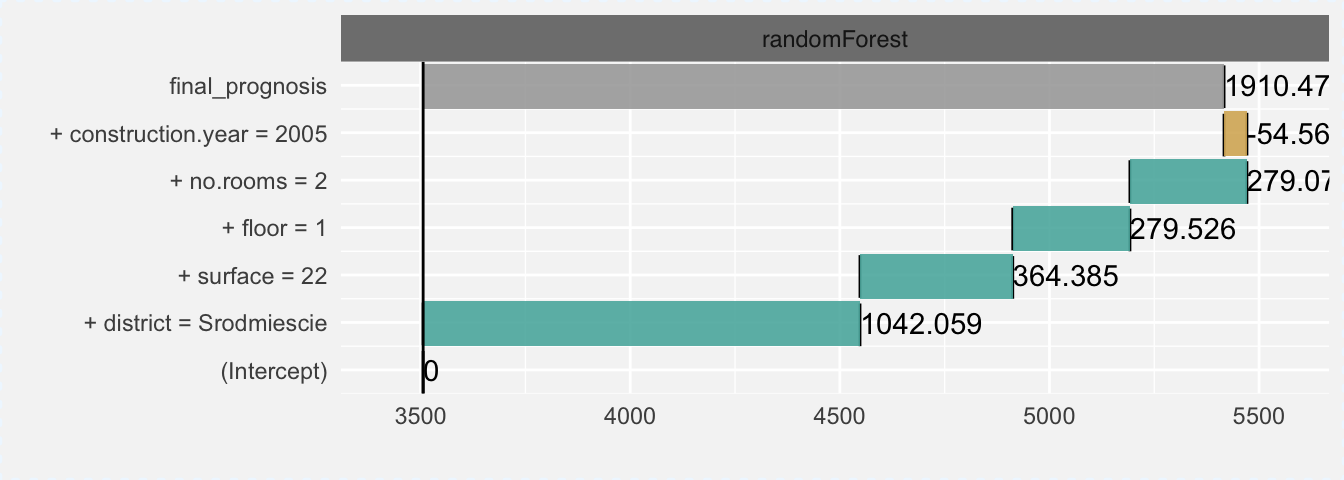
\includegraphics{DALEX_files/figure-latex/single_prediction_break-1.pdf}
\caption{(\#fig:single\_prediction\_break)Break Down Plot for prediction
from the random forest model}
\end{figure}

Both the plot and the table confirm that all variables
(\texttt{district}, \texttt{surface}, \texttt{floor}, \texttt{no.rooms})
have positive effects as expected. Still, these effects are too small
while the final prediction - \texttt{3505\ \ +\ 1881}- is much smaller
than the real price of a square meter \texttt{6679}. Let's see how the
linear model behaves for this observation.

\begin{Shaded}
\begin{Highlighting}[]
\NormalTok{new_apartment_lm <-}\StringTok{ }\KeywordTok{single_prediction}\NormalTok{(explainer_lm, }\DataTypeTok{observation =}\NormalTok{ new_apartment)}
\KeywordTok{plot}\NormalTok{(new_apartment_lm, new_apartment_rf)}
\end{Highlighting}
\end{Shaded}

\begin{figure}
\centering
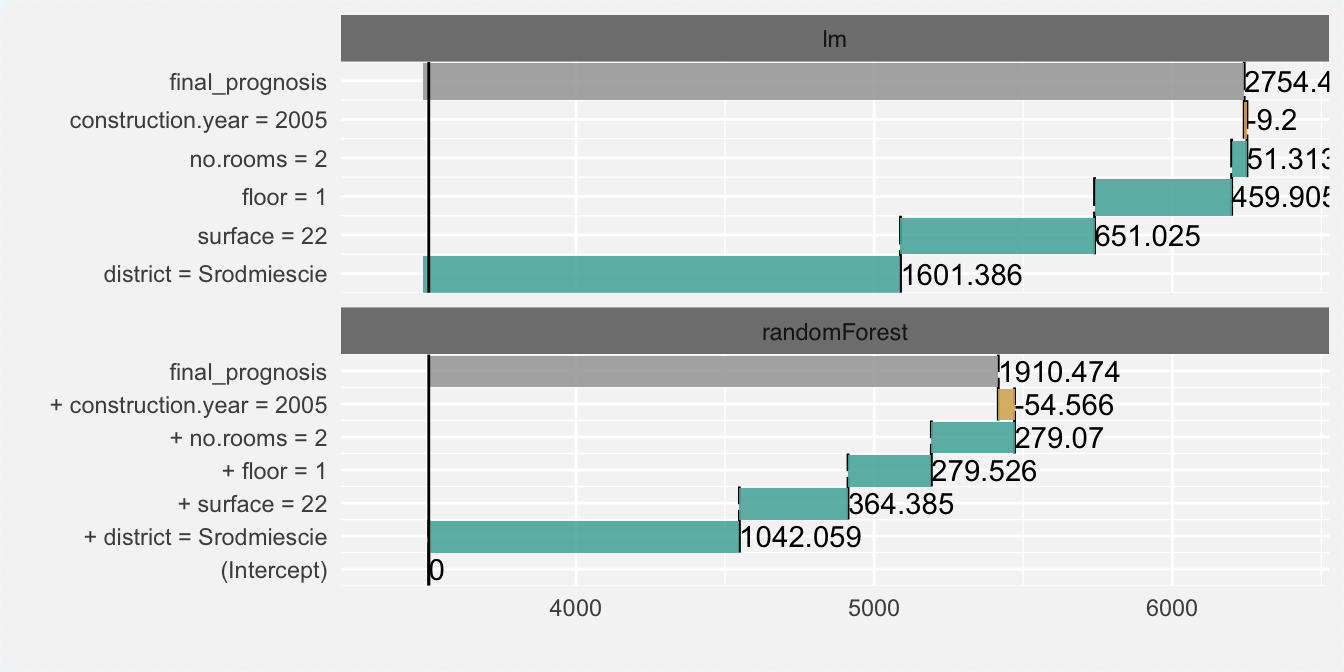
\includegraphics{DALEX_files/figure-latex/single_prediction_break2-1.pdf}
\caption{(\#fig:single\_prediction\_break2)Break Down Plots that compare
the linear model and the random forest model}
\end{figure}

Prediction for linear model is much closer to the real price of square
meter for this apartment.

\hypertarget{epilogue}{%
\chapter{Epilogue}\label{epilogue}}

Let's summarize what has happened in the previous sections.

\begin{itemize}
\tightlist
\item
  Section \ref{useCaseApartmetns} shows two models with equal
  performance for \texttt{apartments} dataset.
\item
  Section \ref{modelPerformance} shows that in general the random forest
  model has smaller residuals than the linear model but there is a small
  fraction of very large residuals.
\item
  Section \ref{outlierDetection} shows that the random forest model
  under-predicts expensive apartments. It is not a model that we would
  like to employ.
\item
  Section \ref{featureImportance} shows that \texttt{construction\_year}
  is important for the random forest model.
\item
  Section \ref{variableResponse} shows that the relation between
  \texttt{construction\_year} and the price of square meter is non
  linear.
\end{itemize}

In this section we showed how to improve the basic linear model by
feature engineering of \texttt{construction\_year}. Findings from the
random forest models will help to create a new feature for the linear
model.

\begin{Shaded}
\begin{Highlighting}[]
\KeywordTok{library}\NormalTok{(}\StringTok{"DALEX"}\NormalTok{)}

\NormalTok{apartments_lm_model_improved <-}\StringTok{ }\KeywordTok{lm}\NormalTok{(m2.price }\OperatorTok{~}\StringTok{ }\KeywordTok{I}\NormalTok{(construction.year }\OperatorTok{<}\StringTok{ }\DecValTok{1935} \OperatorTok{|}\StringTok{ }\NormalTok{construction.year }\OperatorTok{>}\StringTok{ }\DecValTok{1995}\NormalTok{) }\OperatorTok{+}\StringTok{ }\NormalTok{surface }\OperatorTok{+}\StringTok{ }\NormalTok{floor }\OperatorTok{+}\StringTok{ }
\StringTok{                         }\NormalTok{no.rooms }\OperatorTok{+}\StringTok{ }\NormalTok{district, }\DataTypeTok{data =}\NormalTok{ apartments)}

\NormalTok{explainer_lm_improved <-}\StringTok{ }\KeywordTok{explain}\NormalTok{(apartments_lm_model_improved, }
                          \DataTypeTok{data =}\NormalTok{ apartmentsTest[,}\DecValTok{2}\OperatorTok{:}\DecValTok{6}\NormalTok{], }\DataTypeTok{y =}\NormalTok{ apartmentsTest}\OperatorTok{$}\NormalTok{m2.price)}

\NormalTok{mp_lm_improved <-}\StringTok{ }\KeywordTok{model_performance}\NormalTok{(explainer_lm_improved)}
\KeywordTok{plot}\NormalTok{(mp_lm_improved, }\DataTypeTok{geom =} \StringTok{"boxplot"}\NormalTok{)}
\end{Highlighting}
\end{Shaded}

\begin{figure}
\centering
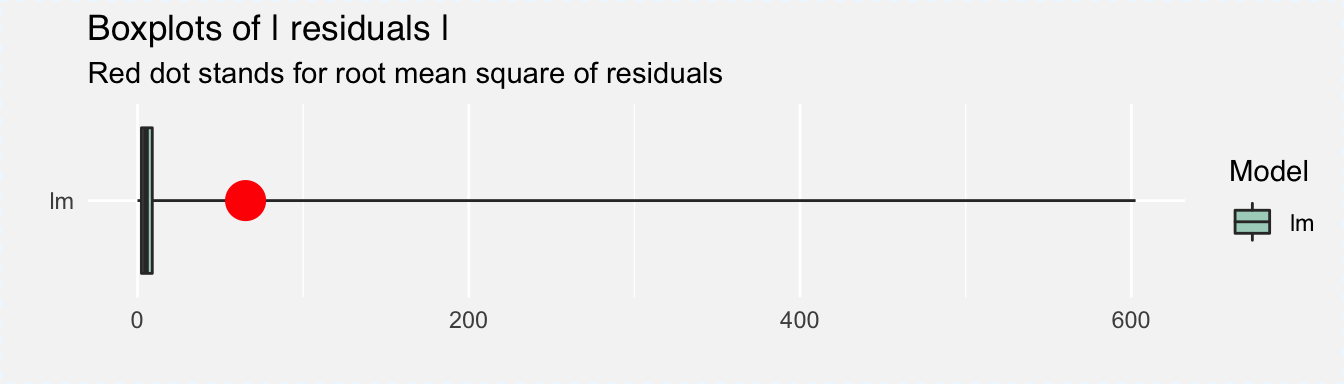
\includegraphics{DALEX_files/figure-latex/final_model-1.pdf}
\caption{(\#fig:final\_model)Distribution of residuals for the new
improved linear model}
\end{figure}

In conclusion, the results presented above prove that the
\texttt{apartments\_lm\_model\_improved} model is much better than the
two initial models introduced in Chapter \ref{modelUnderstanding}.

In this use-case we showed that explainers implemented in DALEX help to
better understand the model and that this knowledge may be used to
create a better final model.

Find more examples, vignietts and cheatsheets at DALEX website
\url{https://github.com/pbiecek/DALEX}.

\hypertarget{exercises}{%
\chapter{Exercises}\label{exercises}}

Examples in previous chapters were based on random forest model and
linear model. But there are so many different approaches for regression
modeling. Try \texttt{gbm} (Generalized Boosted Regression Models),
\texttt{knn} (k-Nearest Neighbour), \texttt{svm} (Support Vector
Machines), \texttt{nnet} (Neural Networks) or other models.

\begin{enumerate}
\def\labelenumi{\arabic{enumi}.}
\tightlist
\item
  Prepare explainers for model performance,
\item
  Prepare explainers for variable importance,
\item
  Prepare explainers for variable response for
  \texttt{construction.year},
\item
  Prepare explainers for model predictions.
\end{enumerate}

Below you will find fits for few different models. Try them out.

\begin{Shaded}
\begin{Highlighting}[]
\KeywordTok{library}\NormalTok{(}\StringTok{"DALEX"}\NormalTok{)}
\KeywordTok{library}\NormalTok{(}\StringTok{"gbm"}\NormalTok{)}

\NormalTok{apartments_gbm_model <-}\StringTok{ }\KeywordTok{gbm}\NormalTok{(m2.price }\OperatorTok{~}\StringTok{ }\NormalTok{construction.year }\OperatorTok{+}\StringTok{ }\NormalTok{surface }\OperatorTok{+}\StringTok{ }\NormalTok{floor }\OperatorTok{+}\StringTok{ }
\StringTok{                         }\NormalTok{no.rooms }\OperatorTok{+}\StringTok{ }\NormalTok{district, }\DataTypeTok{data =}\NormalTok{ apartments, }\DataTypeTok{n.trees =} \DecValTok{1000}\NormalTok{)}
\end{Highlighting}
\end{Shaded}

\begin{verbatim}
## Distribution not specified, assuming gaussian ...
\end{verbatim}

\begin{Shaded}
\begin{Highlighting}[]
\NormalTok{explainer_gbm <-}\StringTok{ }\KeywordTok{explain}\NormalTok{(apartments_gbm_model, }
                          \DataTypeTok{data =}\NormalTok{ apartmentsTest[,}\DecValTok{2}\OperatorTok{:}\DecValTok{6}\NormalTok{], }\DataTypeTok{y =}\NormalTok{ apartmentsTest}\OperatorTok{$}\NormalTok{m2.price,}
                         \DataTypeTok{predict_function =} \ControlFlowTok{function}\NormalTok{(m, d) }\KeywordTok{predict}\NormalTok{(m, d, }\DataTypeTok{n.trees =} \DecValTok{1000}\NormalTok{))}

\KeywordTok{library}\NormalTok{(}\StringTok{"nnet"}\NormalTok{)}
\NormalTok{apartments_nnet_model <-}\StringTok{ }\KeywordTok{nnet}\NormalTok{(m2.price }\OperatorTok{~}\StringTok{ }\NormalTok{construction.year }\OperatorTok{+}\StringTok{ }\NormalTok{surface }\OperatorTok{+}\StringTok{ }\NormalTok{floor }\OperatorTok{+}\StringTok{ }
\StringTok{                         }\NormalTok{no.rooms }\OperatorTok{+}\StringTok{ }\NormalTok{district, }\DataTypeTok{data =}\NormalTok{ apartments,}
                         \DataTypeTok{linout=}\OtherTok{TRUE}\NormalTok{,}
                         \DataTypeTok{size =} \DecValTok{50}\NormalTok{, }\DataTypeTok{maxit=}\DecValTok{100}\NormalTok{)}
\end{Highlighting}
\end{Shaded}

\begin{verbatim}
## # weights:  751
## initial  value 12982043148.246910 
## final  value 821267660.638999 
## converged
\end{verbatim}

\begin{Shaded}
\begin{Highlighting}[]
\NormalTok{explainer_nnet <-}\StringTok{ }\KeywordTok{explain}\NormalTok{(apartments_nnet_model, }
                          \DataTypeTok{data =}\NormalTok{ apartmentsTest[,}\DecValTok{2}\OperatorTok{:}\DecValTok{6}\NormalTok{], }\DataTypeTok{y =}\NormalTok{ apartmentsTest}\OperatorTok{$}\NormalTok{m2.price)}

\KeywordTok{library}\NormalTok{(}\StringTok{"e1071"}\NormalTok{)}
\NormalTok{apartments_svm_model <-}\StringTok{ }\KeywordTok{svm}\NormalTok{(m2.price }\OperatorTok{~}\StringTok{ }\NormalTok{construction.year }\OperatorTok{+}\StringTok{ }\NormalTok{surface }\OperatorTok{+}\StringTok{ }\NormalTok{floor }\OperatorTok{+}\StringTok{ }
\StringTok{                         }\NormalTok{no.rooms }\OperatorTok{+}\StringTok{ }\NormalTok{district, }\DataTypeTok{data =}\NormalTok{ apartments)}

\NormalTok{explainer_svm <-}\StringTok{ }\KeywordTok{explain}\NormalTok{(apartments_svm_model, }
                          \DataTypeTok{data =}\NormalTok{ apartmentsTest[,}\DecValTok{2}\OperatorTok{:}\DecValTok{6}\NormalTok{], }\DataTypeTok{y =}\NormalTok{ apartmentsTest}\OperatorTok{$}\NormalTok{m2.price)}

\KeywordTok{library}\NormalTok{(}\StringTok{"caret"}\NormalTok{)}
\NormalTok{mapartments <-}\StringTok{ }\KeywordTok{model.matrix}\NormalTok{(m2.price }\OperatorTok{~}\StringTok{ }\NormalTok{., }\DataTypeTok{data =}\NormalTok{ apartments)}
\NormalTok{mapartmentsTest <-}\StringTok{ }\KeywordTok{model.matrix}\NormalTok{(m2.price }\OperatorTok{~}\StringTok{ }\NormalTok{., }\DataTypeTok{data =}\NormalTok{ apartmentsTest)}
\NormalTok{apartments_knn_model <-}\StringTok{ }\KeywordTok{knnreg}\NormalTok{(mapartments, apartments[,}\DecValTok{1}\NormalTok{], }\DataTypeTok{k =} \DecValTok{5}\NormalTok{)}

\NormalTok{explainer_knn <-}\StringTok{ }\KeywordTok{explain}\NormalTok{(apartments_knn_model, }
                          \DataTypeTok{data =}\NormalTok{ mapartmentsTest, }\DataTypeTok{y =}\NormalTok{ apartmentsTest}\OperatorTok{$}\NormalTok{m2.price)}

\CommentTok{# Model performance}

\NormalTok{mp_knn <-}\StringTok{ }\KeywordTok{model_performance}\NormalTok{(explainer_knn)}
\NormalTok{mp_svm <-}\StringTok{ }\KeywordTok{model_performance}\NormalTok{(explainer_svm)}
\NormalTok{mp_gbm <-}\StringTok{ }\KeywordTok{model_performance}\NormalTok{(explainer_gbm)}
\NormalTok{mp_nnet <-}\StringTok{ }\KeywordTok{model_performance}\NormalTok{(explainer_nnet)}
\KeywordTok{plot}\NormalTok{(mp_gbm, mp_nnet, mp_svm, mp_knn, }\DataTypeTok{geom =} \StringTok{"boxplot"}\NormalTok{)}
\end{Highlighting}
\end{Shaded}

\begin{figure}
\centering
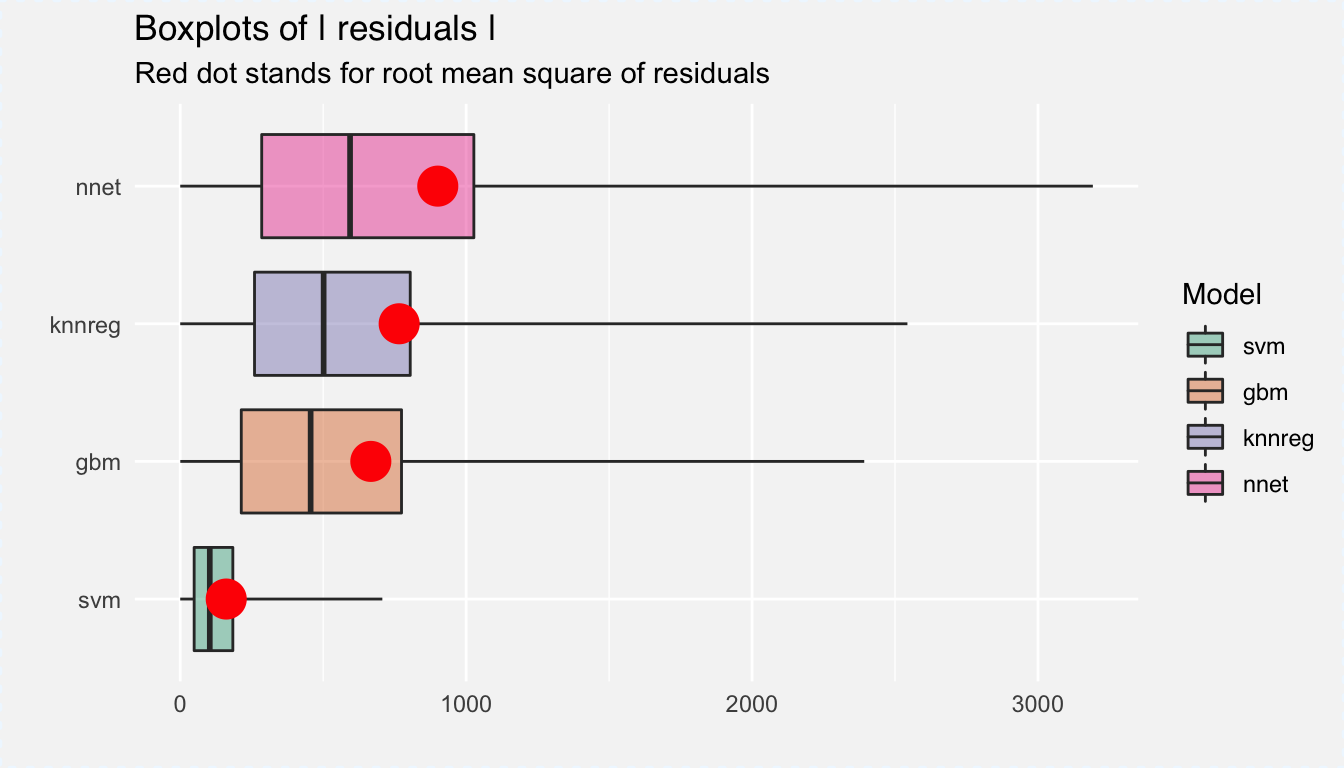
\includegraphics{DALEX_files/figure-latex/Exercises-1.pdf}
\caption{\label{fig:Exercises}Distribution of residuals for fourn new
models}
\end{figure}

\bibliography{book.bib,packages.bib}


\end{document}
